\documentclass[]{beamer}
% \documentclass[table,aspectratio=169]{beamer}
\usepackage{beamerthemesplit}
\usetheme{boxes}
\usecolortheme{seahorse}
% \useinnertheme{myboxes}
% \usepackage{amsmath}
% \usepackage[fleqn]{amsmath}
\usepackage{ifthen}
\usepackage{xspace}
\usepackage{multirow}
\usepackage{booktabs}
\usepackage{xcolor}
\usepackage{changepage}
\usepackage{tabu}
\usepackage[compatibility=false]{caption}
\captionsetup[figure]{font=scriptsize, labelformat=empty, textformat=simple, justification=centering, skip=2pt}

\usepackage{hyperref}
% \hypersetup{pdfborder={0 0 0}, colorlinks=true, urlcolor=black, linkcolor=black, citecolor=black}
\hypersetup{pdfborder={0 0 0}, colorlinks=true, urlcolor=blue, linkcolor=blue, citecolor=blue}

\usepackage[bibstyle=../bib/joaks-slides,maxnames=1,firstinits=true,uniquename=init,backend=biber,bibencoding=utf8]{biblatex}

\newrobustcmd*{\shortfullcite}{\AtNextCite{\renewbibmacro{title}{}\renewbibmacro{in:}{}\renewbibmacro{number}{}}\fullcite}

\newrobustcmd*{\footlessfullcite}{\AtNextCite{\renewbibmacro{title}{}\renewbibmacro{in:}{}}\footfullcite}


% Make all footnotes smaller
%\renewcommand{\footnotesize}{\scriptsize}

\setbeamertemplate{blocks}[rounded][shadow=true]

\setbeamercolor{defaultcolor}{bg=structure!30!normal text.bg,fg=black}
\setbeamercolor{block body}{bg=structure!30!normal text.bg,fg=black}
\setbeamercolor{block title}{bg=structure!50!normal text.bg,fg=black}

% Beamer doesn't play well with enumitem, so hacking some list environments
\newenvironment{mydescription}{
    \begin{description}
        \setlength{\leftskip}{-1.5cm}}
    {\end{description}}

\newenvironment{myitemize}[1][]{
    \begin{itemize}[#1]
        \setlength{\leftskip}{-2.5mm}}
    {\end{itemize}}

\newenvironment{myenumerate}{
    \begin{enumerate}
        \setlength{\leftskip}{-2.5mm}}
    {\end{enumerate}}


\newenvironment<>{varblock}[2][\textwidth]{%
  \setlength{\textwidth}{#1}
  \begin{actionenv}#3%
    \def\insertblocktitle{#2}%
    \par%
    \usebeamertemplate{block begin}}
  {\par%
    \usebeamertemplate{block end}%
  \end{actionenv}}

\newenvironment{displaybox}[1][\textwidth]
{
    \centerline\bgroup\hfill
    \begin{beamerboxesrounded}[lower=defaultcolor,shadow=true,width=#1]{}
}
{
    \end{beamerboxesrounded}\hfill\egroup
}

\newenvironment{onlinebox}[1][4cm]
{
    \newbox\mybox
    \newdimen\myboxht
    \setbox\mybox\hbox\bgroup%
        \begin{beamerboxesrounded}[lower=defaultcolor,shadow=true,width=#1]{}
    \centering
}
{
    \end{beamerboxesrounded}\egroup
    \myboxht\ht\mybox
    \raisebox{-0.25\myboxht}{\usebox\mybox}\hspace{2pt}
}

% footnote without a marker
\newcommand\barefootnote[1]{%
  \begingroup
  \renewcommand\thefootnote{}\footnote{#1}%
  \addtocounter{footnote}{-1}%
  \endgroup
}

% define formatting for footer
\newcommand{\myfootline}{%
    {\it
    \insertshorttitle
    \hspace*{\fill} 
    \insertshortauthor\ -- \insertshortinstitute
    % \ifx\insertsubtitle\@empty\else, \insertshortsubtitle\fi
    \hspace*{\fill}
    \insertframenumber/\inserttotalframenumber}}

% set up footer
\setbeamertemplate{footline}{%
    \usebeamerfont{structure}
    \begin{beamercolorbox}[wd=\paperwidth,ht=2.25ex,dp=1ex]{frametitle}%
        \Tiny\hspace*{4mm}\myfootline\hspace{4mm}
    \end{beamercolorbox}}

% remove navigation bar
\beamertemplatenavigationsymbolsempty

\makeatletter
    \newenvironment{noheadline}{
        \setbeamertemplate{headline}[default]
        \def\beamer@entrycode{\vspace*{-\headheight}}
    }{}
\makeatother

%% Set up color palettes %%%%%%%%%%%%%%%%%%%%%%%%%%%%%%%%%%%%%%%%%%%%
\definecolor{citescol}{RGB}{194,101,1}
%\definecolor{citescol}{RGB}{73,0,165}
\definecolor{urlscol}{RGB}{0,150,206}
%\definecolor{urlscol}{RGB}{0,107,124}
%\definecolor{linkscol}{RGB}{187,24,0}
\definecolor{linkscol}{RGB}{149,0,207}
%\definecolor{linkscol}{RGB}{73,0,165}
\definecolor{mycol}{RGB}{25,23,191}
\definecolor{outputcol}{RGB}{34,139,34}
\definecolor{tcol}{RGB}{165,0,14}

% Color palette GreenOrange_6 from https://jiffyclub.github.io/palettable/tableau/
\definecolor{pgreen}     {RGB}{50,162,81}
\definecolor{porange}    {RGB}{255,127,15}
\definecolor{pblue}      {RGB}{60,183,204}
\definecolor{pyellow}    {RGB}{255,217,74}
\definecolor{pteal}      {RGB}{57,115,124}
\definecolor{pauburn}    {RGB}{184,90,13}
%%%%%%%%%%%%%%%%%%%%%%%%%%%%%%%%%%%%%%%%%%%%%%%%%%%%%%%%%%%%%%%%%%%%%

\usepackage{pgf}
\usepackage{tikz}
\usetikzlibrary{trees,calc,backgrounds,arrows,positioning,automata}

%%%%%%%%%%%%%%%%%%%%%%%%%%%%%%%%%%%%%%%%%%%%%%%%%%%%%%%%%%%%%%%%%%%%%%%%%%%%%%%
% The `conc` macro is the concentration parameter of the Dirichlet process.
% Set it to the desired value here. Delete (or comment out) the `conc` macro to
% leave probability values blank.
\pgfmathsetmacro\conc{0.5}
\pgfmathsetmacro\cconc{10.0}
\pgfmathsetmacro\ccconc{0.5}
\pgfmathsetmacro\disc{0.0}
\pgfmathsetmacro\ddisc{0.5}
\pgfmathsetmacro\dddisc{0.9}
%%%%%%%%%%%%%%%%%%%%%%%%%%%%%%%%%%%%%%%%%%%%%%%%%%%%%%%%%%%%%%%%%%%%%%%%%%%%%%%

% \newcommand{\concentration}{\ensuremath{\alpha}\xspace}
\newcommand{\discount}{\ensuremath{d}\xspace}

\newcommand{\pclass}[3]{%
    \ifthenelse{\equal{#1}{}}%
        {}%
        {\fcolorbox{blue!90}{blue!15}{\catformat{#1}}}%
    \ifthenelse{\equal{#2}{}}%
        {}%
        {\fcolorbox{red!90}{red!15}{\catformat{#2}}}%
    \ifthenelse{\equal{#3}{}}%
        {}%
        {\fcolorbox{gray!90}{gray!15}{\catformat{#3}}}%
}
\newcommand{\catformat}[1]{\textsf{\textbf{#1}}}
\newcommand{\pcat}[3]{%
    \textcolor{blue}{\catformat{#1}}%
    \textcolor{red}{\catformat{#2}}%
    \textcolor{black}{\catformat{#3}}%
}
\newcommand{\branchlabel}[1]{\normalsize #1}
\newcommand{\tiplabel}[1]{\hspace{-0.5em}\normalsize #1}

\newcommand{\calcprob}[2]{%
    \ifthenelse{\isundefined{\conc}}%
        {}%
        {\pgfmathparse{(#1/(\conc+1))*(#2/(\conc+2))}\pgfmathprintnumber{\pgfmathresult}}%
}
\newcommand{\ccalcprob}[2]{%
    \ifthenelse{\isundefined{\cconc}}%
        {}%
        {\pgfmathparse{(#1/(\cconc+1))*(#2/(\cconc+2))}\pgfmathprintnumber{\pgfmathresult}}%
}
\newcommand{\cccalcprob}[2]{%
    \ifthenelse{\isundefined{\ccconc}}%
        {}%
        {\pgfmathparse{(#1/(\ccconc+1))*(#2/(\ccconc+2))}\pgfmathprintnumber{\pgfmathresult}}%
}

\newcommand{\getconc}[1]{%
    \ifthenelse{\isundefined{\conc}}%
        {}%
        {\conc}%
}
\newcommand{\getdisc}[1]{%
    \ifthenelse{\isundefined{\disc}}%
        {}%
        {\disc}%
}

% \tikzset{hide on/.code={\only<#1>{\color{fg!20}}}}
\tikzset{hide on/.code={\only<#1>{\color{white}}}}
\tikzset{
    invisible/.style={opacity=0},
    visible on/.style={alt={#1{}{invisible}}},
    alt/.code args={<#1>#2#3}{%
        \alt<#1>{\pgfkeysalso{#2}}{\pgfkeysalso{#3}}
        % \pgfkeysalso doesn't change the path
    },
}


\newcommand{\citationNeeded}{\textcolor{magenta}{\textbf{[CITATION NEEDED!]}}\xspace}
\newcommand{\tableNeeded}{\textcolor{magenta}{\textbf{[TABLE NEEDED!]}}\xspace}
\newcommand{\figureNeeded}{\textcolor{magenta}{\textbf{[FIGURE NEEDED!]}}\xspace}
\newcommand{\highLight}[1]{\textcolor{magenta}{\MakeUppercase{#1}}}

\newcommand{\datasets}{data sets\xspace}
\newcommand{\dataset}{data set\xspace}

\newcommand{\editorialNote}[1]{\textcolor{red}{[\textit{#1}]}}
\newcommand{\ignore}[1]{}
\newcommand{\addTail}[1]{\textit{#1}.---}
\newcommand{\super}[1]{\ensuremath{^{\textrm{#1}}}}
\newcommand{\sub}[1]{\ensuremath{_{\textrm{#1}}}}
\newcommand{\dC}{\ensuremath{^\circ{\textrm{C}}}}
\newcommand{\tb}{\hspace{2em}}
\newcommand{\tn}{\tabularnewline}
\newcommand{\spp}[1]{\textit{#1}}

\providecommand{\e}[1]{\ensuremath{\times 10^{#1}}}

\newcommand{\change}[2]{{\color{red} #2}\xspace}
\newcommand{\thought}[1]{\textcolor{purple}{THOUGHT: #1}}

\newcommand{\widthFigure}[5]{\begin{figure}[htbp]
\begin{center}
    \includegraphics[width=#1\textwidth]{#2}
    \captionsetup{#3}
    \caption{#4}
    \label{#5}
    \end{center}
    \end{figure}}

\newcommand{\heightFigure}[5]{\begin{figure}[htbp]
\begin{center}
    \includegraphics[height=#1\textheight]{#2}
    \captionsetup{#3}
    \caption{#4}
    \label{#5}
    \end{center}
    \end{figure}}

\newcommand{\smartFigure}[4]{%
    \begin{figure}[htbp]
        \begin{center}
            \includegraphics[width=\textwidth,height=0.95\textheight,keepaspectratio]{#1}
            \captionsetup{#2}
            \caption{#3}
            \label{#4}
        \end{center}
    \end{figure}
}

\newcommand{\mFigure}[3]{\smartFigure{#1}{listformat=figList}{#2}{#3}\clearpage}
\newcommand{\embedHeightFigure}[4]{\heightFigure{#1}{#2}{listformat=figList}{#3}{#4}}
\newcommand{\embedWidthFigure}[4]{\widthFigure{#1}{#2}{listformat=figList}{#3}{#4}}
\newcommand{\siFigure}[3]{\smartFigure{#1}{name=Figure S, labelformat=noSpace, listformat=sFigList}{#2}{#3}\clearpage}

\newcommand{\validationfiguregriddescription}{The first four columns show the
    results from different distributions on the relative effective size of the
    ancestral population, decreasing in variance from left to right.
    The fifth column shows results when the effective size
    ($\epopsize{}\murate{}$) of all populations is fixed to 0.002.
    For the first two and last two rows, the simulated character matrix for
    each population had 500,000 and 100,000 characters, respectively.
    The first and third rows show the results of analyses using all characters,
    whereas the second and fourth rows show the results when only variable
    characters are used.
}
\newcommand{\missingdatafigurecolumndescription}{The columns, from left to
    right, show the results when each simulated 500,000-character matrix has
    approximately 0\%, 10\%, 25\%, and 50\% missing cells.
}
\newcommand{\comparisoncolumndescription}[2]{
    For comparison, the first column shows the results of the 500 \datasets from
    Figure~#1\ref{#2}; the remaining columns show the results of
    100 \datasets.
}
\newcommand{\missingdatafigurerowdescription}{The rows show the results when
    (top) all sites and (bottom) only variable sites are analyzed.
}
\newcommand{\filtereddatafigurecolumndescription}{The columns, from left to
    right, show the results when each simulated
    500,000-character \dataset has a probability of 100\%, 80\%, 60\%, and 40\%
    of sampling each simulated singleton pattern.
    E.g., each character matrix analyzed in the far right column is missing
    approximately 60\% of characters where all but one gene copy has the same
    allele.
}
\newcommand{\filtereddatafigurerowdescription}{The rows show the results when
    (top) all sites and (bottom) only variable sites are analyzed.
}
\newcommand{\weusedmatplotlib}{We generated the plot using matplotlib Version
    2.0.0 \citep{matplotlib}.}
\newcommand{\weusedggplot}{We generated the plots with ggplot2 Version 2.2.1
    \citep{ggplot2}.}
\newcommand{\weusedggridges}{We generated the plots with ggridges Version 0.4.1
    \citep{ggridges041} and ggplot2 Version 2.2.1 \citep{ggplot2}.}
\newcommand{\neventplotannotations}{For each plot,
    the proportion of \datasets for which the number of events with the largest
    posterior probability matched the true number of events---$p(\hat{\nevents}
    = \nevents)$---is shown in the upper left corner,
    the median posterior probability of the correct number of events across all
    \datasets---$\widetilde{p(\nevents|\alldata)}$---is shown in the upper
    right corner, and
    the proportion of \datasets for which the true divergence model was
    included in the 95\% credible set---$p(\nevents \in
    \textrm{CS})$---is shown in the lower right.
}
\newcommand{\accuracyscatterplotannotations}[1]{For each plot, the
    root-mean-square error (RMSE) and the proportion of estimates for which the
    95\% credible interval contained the true value---$p(#1 \in
    \textrm{CI})$---is given.
}
\newcommand{\neventsshadingdescription}{The number of \datasets that fall
    within each possible cell of true versus estimated numbers of events is
    shown, and cells with more \datasets are shaded darker.
}

%% macro to make long strings breakable over lines
\makeatletter
\def\breakable#1{\xHyphen@te#1$\unskip}
\def\xHyphen@te{\@ifnextchar${\@gobble}{\sw@p{\allowbreak{}\xHyphen@te}}}
% \def\xHyphen@te{\@ifnextchar${\@gobble}{\sw@p{\hskip 0pt plus 1pt\xHyphen@te}}}
\def\sw@p#1#2{#2#1}
\makeatother

\newcommand{\given}{\ensuremath{\,|\,}\xspace}
\newcommand{\pr}{\ensuremath{p}}

\newcommand{\data}{\ensuremath{D}\xspace}
\newcommand{\model}[1][]{\ensuremath{M_{#1}}\xspace}
\newcommand{\parameters}[1][]{\ensuremath{\Theta_{#1}}\xspace}
\newcommand{\parameter}[1][]{\ensuremath{\theta_{#1}}\xspace}
\newcommand{\diff}[1]{\ensuremath{\mathrm{d}#1}}

\newcommand{\distgamma}{\ensuremath{\textrm{Gamma}}\xspace}
\newcommand{\distexponential}{\ensuremath{\textrm{Exponential}}\xspace}
\newcommand{\dgamma}[2]{\ensuremath{\distgamma(\textrm{shape} = #1, \textrm{mean} = #2)}}
\newcommand{\dexponential}[1]{\ensuremath{\distexponential(\textrm{mean} = #1)}}

\newcommand{\ncomparisons}{\ensuremath{n\xspace}}
\newcommand{\nevents}[1][]{\ensuremath{k_{#1}\xspace}}
\newcommand{\nloci}[1][]{\ensuremath{m_{#1}\xspace}}

\newcommand{\observedallelecount}[1][]{\ensuremath{n_{#1}}\xspace}
\newcommand{\observedredallelecount}[1][]{\ensuremath{r_{#1}}\xspace}

\newcommand{\nodeallelecount}[2]{\ensuremath{n_{#1}^{#2}}}
\newcommand{\noderedallelecount}[2]{\ensuremath{r_{#1}^{#2}}}

\newcommand{\allelecount}[1][]{\ensuremath{\nodeallelecount{#1}{}}\xspace}
\newcommand{\redallelecount}[1][]{\ensuremath{\noderedallelecount{#1}{}}\xspace}

\newcommand{\leafallelecounts}[1][]{\ensuremath{\mathbf{n}_{#1}}\xspace}
\newcommand{\leafredallelecounts}[1][]{\ensuremath{\mathbf{r}_{#1}}\xspace}
\newcommand{\maxleafallelecounts}{\ensuremath{\textrm{max}(\mathbf{n})}\xspace}

\newcommand{\comparisondata}[1][]{\ensuremath{D_{#1}}\xspace}
\newcommand{\alldata}[1][]{\ensuremath{\mathbf{D}}\xspace}

\newcommand{\branchindex}{\ensuremath{x}\xspace}
\newcommand{\allelecountbottom}[1][\branchindex]{\nodeallelecount{#1}{B}}
\newcommand{\allelecounttop}[1][\branchindex]{\nodeallelecount{#1}{T}}
\newcommand{\redallelecountbottom}[1][\branchindex]{\noderedallelecount{#1}{B}}
\newcommand{\redallelecounttop}[1][\branchindex]{\noderedallelecount{#1}{T}}

\newcommand{\dppmsbayes}{\upshape\texttt{dpp-msbayes}\xspace}
\newcommand{\cpp}{\upshape\texttt{C++}\xspace}
\newcommand{\ecoevolity}{\upshape\texttt{ecoevolity}\xspace}
\newcommand{\timesizeratemixer}{\upshape\texttt{TimeSizeRateMixer}\xspace}
\newcommand{\timerootsizemixer}{\upshape\texttt{TimeRootSizeMixer}\xspace}
\newcommand{\simcoevolity}{\upshape\texttt{simcoevolity}\xspace}
\newcommand{\sumcoevolity}{\upshape\texttt{sumcoevolity}\xspace}
\newcommand{\pycoevolity}{\upshape\texttt{pycoevolity}\xspace}

\newcommand{\rgmurate}{\ensuremath{u}\xspace}
\newcommand{\grmurate}{\ensuremath{v}\xspace}
\newcommand{\murate}[1][]{\ensuremath{\mu_{#1}}\xspace}
\newcommand{\murates}[1][]{\ensuremath{\boldsymbol{\mu}_{#1}}\xspace}
\newcommand{\gfreq}[1][]{\ensuremath{\pi_{#1}}\xspace}
\newcommand{\gfreqs}[1][]{\ensuremath{\boldsymbol{\pi}_{#1}}\xspace}

\newcommand{\comparisondivtime}[1][]{\ensuremath{t_{#1}}\xspace}
\newcommand{\comparisondivtimes}[1][]{\ensuremath{\mathbf{t}_{#1}}\xspace}
\newcommand{\divtime}[1][]{\ensuremath{\tau_{#1}}\xspace}
\newcommand{\divtimes}[1][]{\ensuremath{\boldsymbol{\tau}_{#1}}\xspace}
\newcommand{\divtimemodel}[1][]{\ensuremath{T_{#1}}\xspace}
\newcommand{\divtimesets}{\ensuremath{\mathcal{T}}\xspace}
\newcommand{\genetree}[1][]{\ensuremath{g_{#1}}\xspace}
\newcommand{\sptree}[1][]{\ensuremath{S_{#1}}\xspace}
\newcommand{\sptrees}[1][]{\ensuremath{\mathbf{S}_{#1}}\xspace}

\newcommand{\descendantpopindex}[1]{\ensuremath{D{#1}}}
\newcommand{\rootpopindex}[1][]{\ensuremath{R{#1}}\xspace}
\newcommand{\epopsize}[1][]{\ensuremath{N_{e}^{#1}}\xspace}
\newcommand{\sepopsize}[1][]{\ensuremath{N}\xspace}
\newcommand{\comparisonpopsizes}[1][]{\ensuremath{\mathbb{N}_{e}{#1}}\xspace}
\newcommand{\collectionpopsizes}[1][]{\ensuremath{\mathbf{N_{e}}_{#1}}\xspace}
\newcommand{\rootrelativepopsize}{\ensuremath{R_{\epopsize[\rootpopindex]}}\xspace}

\newcommand{\dirp}{\ensuremath{\textrm{DP}}\xspace}
\newcommand{\concentration}{\ensuremath{\alpha}\xspace}
\newcommand{\basedistribution}{\ensuremath{H}\xspace}
\newcommand{\gshape}{\ensuremath{k}\xspace}
\newcommand{\gscale}{\ensuremath{\theta}\xspace}

\newcommand{\multiplier}{\ensuremath{m}\xspace}
\newcommand{\proposed}{\ensuremath{^{\prime}}\xspace}
\newcommand{\tuningparameter}{\ensuremath{\lambda}\xspace}
\newcommand{\uniformdeviate}{\ensuremath{u}\xspace}
\newcommand{\sizechange}{\ensuremath{\delta}\xspace}

\newcommand\mybullet{\leavevmode%
\usebeamertemplate{itemize item}\hspace{.5em}}

\makeatletter
\newcommand*{\rom}[1]{\expandafter\@slowromancap\romannumeral #1@}
\makeatother

\newcommand{\blankslide}{{\setbeamercolor{background canvas}{bg=black}
\setbeamercolor{whitetext}{fg=white}
\begin{frame}<handout:0>[plain]
\end{frame}}}

\newcommand{\whiteslide}{
\begin{frame}<handout:0>[plain]
\end{frame}}


\newcommand{\ifTwoArgs}[3]{\ifthenelse{\equal{#1}{}\or\equal{#2}{}}{}{#3}\xspace}
\newcommand{\divModel}[1]{\ensuremath{m_{#1}}\xspace}
\newcommand{\divTimeMap}[1]{\ensuremath{T_{#1}}\xspace}
\newcommand{\alignment}[2]{\ensuremath{X_{#1\protect\ifTwoArgs{#1}{#2}{,}#2}}\xspace}
\newcommand{\divTimeMapVector}{\ensuremath{\mathbf{\divTimeMap{}}}\xspace}
\newcommand{\alignmentVector}{\ensuremath{\mathbf{\alignment{}{}}}\xspace}
\newcommand{\allParameters}[1]{\ensuremath{\theta_{#1}}\xspace}
\newcommand{\flipdata}{\ensuremath{D}\xspace}
\newcommand{\coinmodel}[1][]{\ensuremath{M_{#1}}\xspace}
\newcommand{\probheads}[1][]{\ensuremath{\theta_{#1}}\xspace}
\newcommand{\nmodels}{\ensuremath{N}\xspace}


\newcommand{\nucleotideformat}[1]
{\tiny
    \begin{minipage}[c][1.1ex][c]{1.1ex}
        % \vspace{-0.9ex}
        % \begin{center}
            % \hspace{-0.7ex}
            \centering{#1}
        % \end{center}
    \end{minipage}
}

% \newcommand{\nA}{\textcolor{red}{A}}
% \newcommand{\nC}{\textcolor{green}{C}}
% \newcommand{\nG}{\textcolor{yellow}{G}}
% \newcommand{\nT}{\textcolor{blue}{T}}
\newcommand{\nA}{\nucleotideformat{A}}
\newcommand{\nC}{\nucleotideformat{C}}
\newcommand{\nG}{\nucleotideformat{G}}
\newcommand{\nT}{\nucleotideformat{T}}

%% Dimensions and macros to calc frame content width and height
\newif\ifsidebartheme
\sidebarthemetrue

\newlength\frametextheight
\newlength\headlessframetextheight
\setlength{\frametextheight}{0.88\textheight}
\setlength{\headlessframetextheight}{1\textheight}

\newdimen\smarttextheight
\newdimen\contentheight
\newdimen\contentwidth
\newdimen\contentleft
\newdimen\contentbottom
\makeatletter
\newcommand*{\calculatespace}{%
\contentheight=\paperheight%
\ifx\beamer@frametitle\@empty%
    \setbox\@tempboxa=\box\voidb@x%
  \else%
    \setbox\@tempboxa=\vbox{%
      \vbox{}%
      {\parskip0pt\usebeamertemplate***{frametitle}}%
    }%
    \ifsidebartheme%
      \advance\contentheight by-1em%
    \fi%
  \fi%
\advance\contentheight by-\ht\@tempboxa%
\advance\contentheight by-\dp\@tempboxa%
\advance\contentheight by-\beamer@frametopskip%
\ifbeamer@plainframe%
\contentbottom=0pt%
\else%
\advance\contentheight by-\headheight%
\advance\contentheight by\headdp%
\advance\contentheight by-\footheight%
\advance\contentheight by4pt%
\contentbottom=\footheight%
\advance\contentbottom by-4pt%
\fi%
\contentwidth=\paperwidth%
\ifbeamer@plainframe%
\contentleft=0pt%
\else%
\advance\contentwidth by-\beamer@rightsidebar%
\advance\contentwidth by-\beamer@leftsidebar\relax%
\contentleft=\beamer@leftsidebar%
\fi%
\smarttextheight=\contentheight%
\advance\smarttextheight by-4mm%
\ifx\beamer@frametitle\@empty%
    \advance\smarttextheight by-3mm%
\fi%
}
\makeatother

\newcommand{\smartgraphic}[3][\frametextheight]{%
\includegraphics#2[width=\linewidth,height=#1,keepaspectratio]{#3}%
}

\bibliography{../bib/references}

\title[Phyletica Lab Project]{Phyletica Lab Simulation Project}

\author[Jamie Oaks]{
    Jamie R.\ Oaks}

\institute[\href{http://phyletica.org}{phyletica.org}]{
    % \inst{1}%
    Department of Biological Sciences \&
    % \inst{2}
    Museum of Natural History,
    Auburn University
}

% \date{\today}
\date{January 29, 2020}


\setbeamersize{text margin left=3mm, text margin right=3mm}

\begin{document}

% \maketitle

\begin{frame}
    \begin{columns}

        \column{.49\textwidth}

        \vspace{-2cm}
        \begin{minipage}[c][\headlessframetextheight][c]{0.98\columnwidth}
            \maketitle
        \end{minipage}

        \column{.49\textwidth}

        \begin{minipage}[t][\headlessframetextheight][c]{\columnwidth}
            \begin{figure}
                \begin{center}
                    \smartgraphic[\headlessframetextheight]{}{../images/darwin-tol-copyright-boris-kulikov-2007.jpg}
                \vspace{-2.0mm}
                \caption{\tiny \copyright~2007 Boris Kulikov \href{http://boris-kulikov.blogspot.com/}{boris-kulikov.blogspot.com}}
                \end{center}
            \end{figure}
        \end{minipage}
    \end{columns}
\end{frame}



% \input{intro-general.tex}

% \input{intro-shared-divs.tex}

% \begin{frame}[c]
    \frametitle{Violating independent divergences}

%% This is a tikz file
\tikzset{node lower left/.style={font=\small,anchor=north east,text height=0.240cm,text depth=0.068cm,inner sep=0.03cm},
leaf/.style={font=\small,anchor=west,text height=0.240cm,text depth=0.068cm},
node upper left/.style={font=\small,anchor=south east,text height=0.240cm,text depth=0.068cm,inner sep=0.03cm},
bracket label/.style={font=\small,anchor=west,text height=0.240cm,text depth=0.068cm,inner sep=0.1cm},
node upper right/.style={font=\small,anchor=south west,text height=0.240cm,text depth=0.068cm,inner sep=0.03cm},
node right/.style={font=\small,anchor=west,text height=0.240cm,text depth=0.068cm,inner sep=0.03cm},
branch/.style={font=\tiny,text height=0.144cm,text depth=0.041cm,inner sep=0.025cm},
root/.style={font=\small,anchor=east,text height=0.240cm,text depth=0.068cm},
node lower right/.style={font=\small,anchor=north west,text height=0.240cm,text depth=0.068cm,inner sep=0.03cm}}

\centering{
\resizebox{!}{\frametextheight}{%
\begin{tikzpicture}[ultra thick,inner sep=0.1cm]
%  4:\hspace{20mm}\includegraphics[width=15mm,resolution=150]{../images/phylopics/gekko-vittatus-4-yellow-shadow.png}
%  3
% +2:\hspace{20mm}
\includegraphics[width=15mm,resolution=150]{../images/phylopics/gekko-vittatus-5-teal-shadow.png}
% ||
% |6:\hspace{20mm}
\includegraphics[width=15mm,resolution=150]{../images/phylopics/gekko-vittatus-6-auburn-shadow.png}
% |
% |10:\hspace{20mm}\includegraphics[width=15mm,resolution=150]{../images/phylopics/gecko-pixabay-cc0-4-yellow-shadow.png}
% 09
% |81:\hspace{20mm}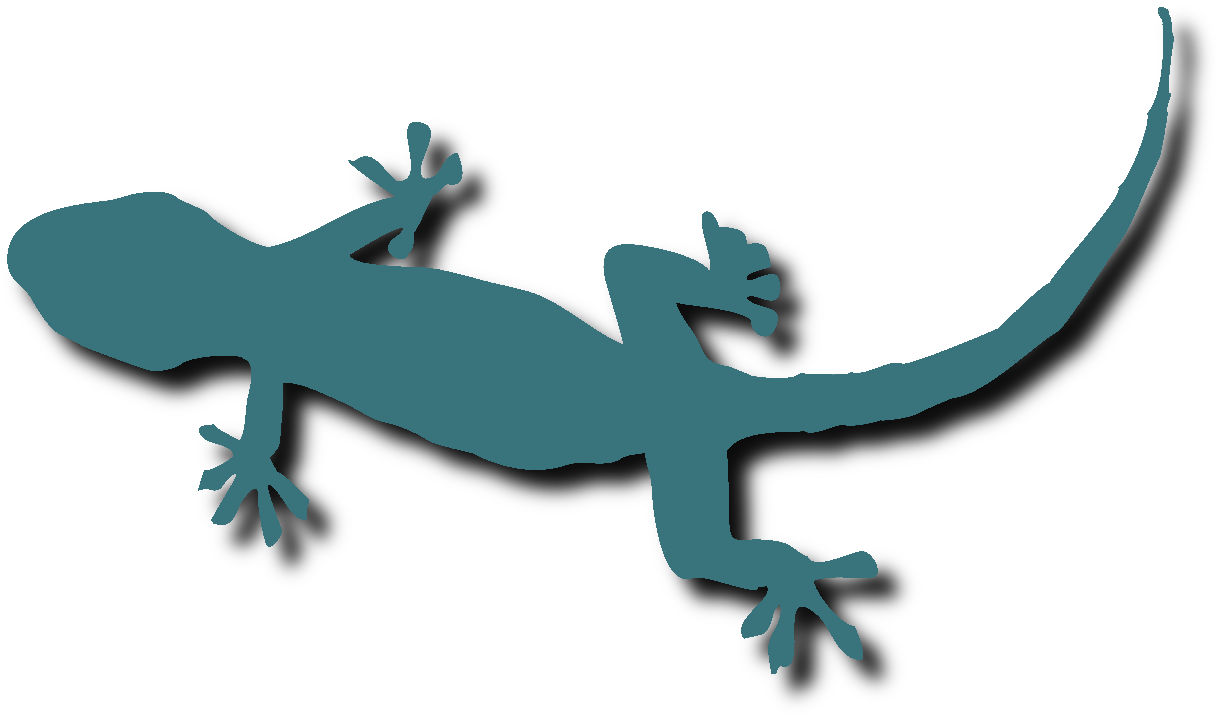
\includegraphics[width=15mm,resolution=150]{../images/phylopics/gecko-pixabay-cc0-5-teal-shadow.png}
% ||
% |12:\hspace{20mm}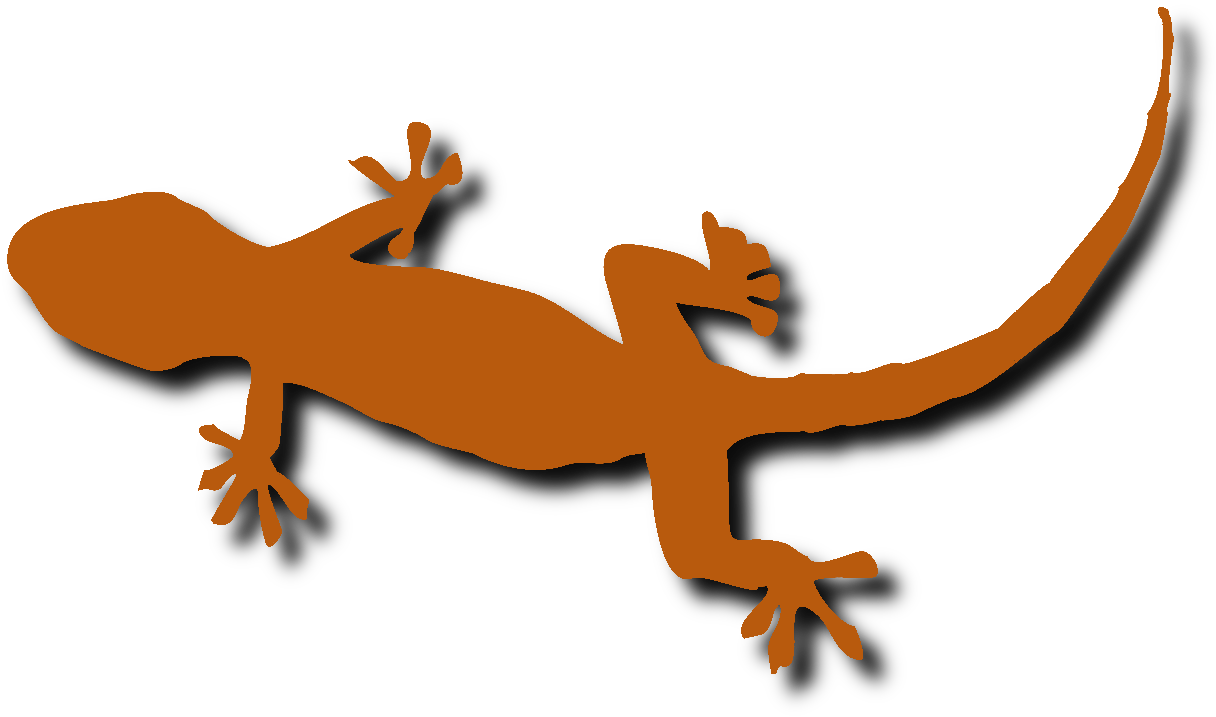
\includegraphics[width=15mm,resolution=150]{../images/phylopics/gecko-pixabay-cc0-6-auburn-shadow.png}
% 7
% |15:\hspace{20mm}\includegraphics[width=15mm,resolution=150]{../images/phylopics/gekko-gecko-4-yellow-shadow.png}
% |14
% +13:\hspace{20mm}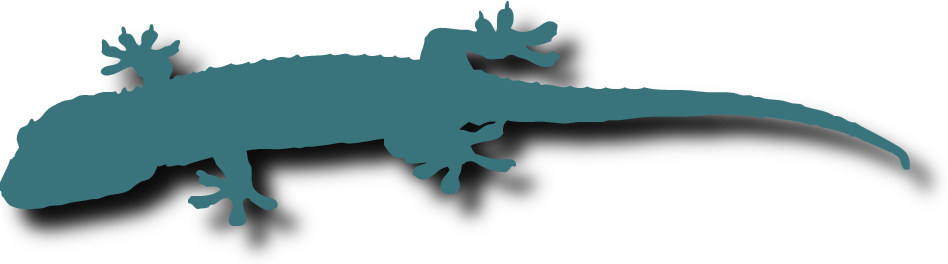
\includegraphics[width=15mm,resolution=150]{../images/phylopics/gekko-gecko-5-teal-shadow.png}
%  |
%  17:\hspace{20mm}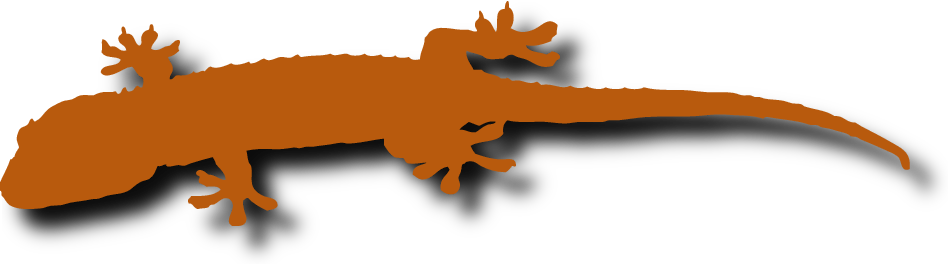
\includegraphics[width=15mm,resolution=150]{../images/phylopics/gekko-gecko-6-auburn-shadow.png}

% The scale is 1.000000, and the yScale is 0.800000

%% Coordinates of nodes.
\coordinate (island) at (11.6, 3.2);
\node[visible on=<1>] at (island) {\includegraphics[height=8.0cm,resolution=300]{../images/islands-1.pdf}};
\node[visible on=<2>] at (island) {\includegraphics[height=8.0cm,resolution=300]{../images/islands-3-bare.pdf}};
\node[visible on=<3>] at (island) {\includegraphics[height=8.0cm,resolution=300]{../images/islands-1.pdf}};
\node[visible on=<4>] at (island) {\includegraphics[height=8.0cm,resolution=300]{../images/islands-2.pdf}};
\node[visible on=<5->] at (island) {\includegraphics[height=8.0cm,resolution=300]{../images/islands-3.pdf}};

\draw [visible on=<5->, pteal,very thick,dashed] (6.600,-0.300) -- (6.600,6.728);
% \node [font=\LARGE,yshift=-0.200cm,text height=0.415cm,text depth=0.118cm] at (6.600,-0.300) {\color{pteal}$\tau_{\scriptscriptstyle 1}$};
\draw [visible on=<4->, pauburn,very thick,dashed] (4.600,-0.300) -- (4.600,6.728);
% \node [font=\LARGE,yshift=-0.200cm,text height=0.415cm,text depth=0.118cm] at (4.600,-0.300) {\color{pauburn}$\tau_{\scriptscriptstyle 2}$};
\draw [visible on=<2->, pteal,very thick,dashed] (0.100,-0.300) -- (0.100,6.728);
% \node [font=\LARGE,yshift=-0.200cm,text height=0.415cm,text depth=0.118cm] at (0.100,-0.300) {\color{pteal}$\tau_{\scriptscriptstyle 3}$};
\coordinate (n0) at (0.000,3.600);
\coordinate (n1) at (0.100,3.600);
\coordinate (n1p) at (0.000,3.600);
\coordinate (n2) at (4.600,5.400);
\coordinate (n2h) at (3.200,5.400);
\coordinate (n2c) at (1.600,5.400);
\coordinate (n2p) at (0.100,5.400);
\coordinate (n3) at (6.600,6.000);
\coordinate (n3p) at (4.600,6.000);
\coordinate (n3h) at (5.500,6.000);
\coordinate (n4) at (7.100,6.400);
\coordinate (n4p) at (6.600,6.400);
\coordinate (n5) at (7.100,5.600);
\coordinate (n5p) at (6.600,5.600);
\coordinate (n6) at (7.100,4.800);
\coordinate (n6p) at (4.600,4.800);
\coordinate (n6h) at (5.500,4.800);
\coordinate (n7) at (0.100,1.800);
\coordinate (n7p) at (0.100,1.800);
\coordinate (n8) at (4.600,3.000);
\coordinate (n8h) at (3.200,3.000);
\coordinate (n8c) at (1.600,3.000);
\coordinate (n8p) at (0.100,3.000);
\coordinate (n9) at (6.600,3.600);
\coordinate (n9p) at (4.600,3.600);
\coordinate (n9h) at (5.500,3.600);
\coordinate (n10) at (7.100,4.000);
\coordinate (n10p) at (6.600,4.000);
\coordinate (n11) at (7.100,3.200);
\coordinate (n11p) at (6.600,3.200);
\coordinate (n12) at (7.100,2.400);
\coordinate (n12p) at (4.600,2.400);
\coordinate (n12h) at (5.500,2.400);
\coordinate (n13) at (4.600,0.600);
\coordinate (n13h) at (3.200,0.600);
\coordinate (n13c) at (1.600,0.600);
\coordinate (n13p) at (0.100,0.600);
\coordinate (n14) at (6.600,1.200);
\coordinate (n14p) at (4.600,1.200);
\coordinate (n14h) at (5.500,1.200);
\coordinate (n15) at (7.100,1.600);
\coordinate (n15p) at (6.600,1.600);
\coordinate (n16) at (7.100,0.800);
\coordinate (n16p) at (6.600,0.800);
\coordinate (n17) at (7.100,0.000);
\coordinate (n17p) at (4.600,0.000);
\coordinate (n17h) at (5.500,0.000);

%% horizontal lines
\draw [visible on=<2->] (n1p) -- (n1);
\draw [visible on=<2>] (n2p) -- (n2c);
\draw [visible on=<3>] (n2p) -- (n2h);
\draw [visible on=<4->] (n2p) -- (n2);
\draw [visible on=<5->] (n3p) -- (n3);
\draw [visible on=<4>] (n3p) -- (n3h);
\draw [visible on=<5->] (n4p) -- (n4);
\draw [visible on=<5->] (n5p) -- (n5);
\draw [visible on=<5->] (n6p) -- (n6);
\draw [visible on=<4>] (n6p) -- (n6h);
\draw [visible on=<2->] (n7p) -- (n7);
\draw [visible on=<2>] (n8p) -- (n8c);
\draw [visible on=<3>] (n8p) -- (n8h);
\draw [visible on=<4->] (n8p) -- (n8);
\draw [visible on=<5->] (n9p) -- (n9);
\draw [visible on=<4>] (n9p) -- (n9h);
\draw [visible on=<5->] (n10p) -- (n10);
\draw [visible on=<5->] (n11p) -- (n11);
\draw [visible on=<5->] (n12p) -- (n12);
\draw [visible on=<4>] (n12p) -- (n12h);
\draw [visible on=<2>] (n13p) -- (n13c);
\draw [visible on=<3>] (n13p) -- (n13h);
\draw [visible on=<4->] (n13p) -- (n13);
\draw [visible on=<5->] (n14p) -- (n14);
\draw [visible on=<4>] (n14p) -- (n14h);
\draw [visible on=<5->] (n15p) -- (n15);
\draw [visible on=<5->] (n16p) -- (n16);
\draw [visible on=<5->] (n17p) -- (n17);
\draw [visible on=<4>] (n17p) -- (n17h);

%% vertical lines
\draw [visible on=<2->,line cap=rect] (n2p) -- (n7p);
\draw [visible on=<4->,line cap=rect] (n3p) -- (n6p);
\draw [visible on=<5->,line cap=rect] (n4p) -- (n5p);
\draw [visible on=<2->,line cap=rect] (n8p) -- (n13p);
\draw [visible on=<4->,line cap=rect] (n9p) -- (n12p);
\draw [visible on=<5->,line cap=rect] (n10p) -- (n11p);
\draw [visible on=<4->,line cap=rect] (n14p) -- (n17p);
\draw [visible on=<5->,line cap=rect] (n15p) -- (n16p);

%% leaf labels
\node [visible on=<1>] at (n8p) {\hspace{20mm}
\includegraphics[width=15mm,resolution=150]{../images/phylopics/gekko-vittatus-5-teal-shadow.png}};

\node [visible on=<2>] at (n2c) {\hspace{20mm}
\includegraphics[width=15mm,resolution=150]{../images/phylopics/gekko-vittatus-5-teal-shadow.png}};
\node [visible on=<2>] at (n8c) {\hspace{20mm}\includegraphics[width=15mm,resolution=150]{../images/phylopics/gekko-vittatus-4-yellow-shadow.png}};
\node [visible on=<2>] at (n13c) {\hspace{20mm}
\includegraphics[width=15mm,resolution=150]{../images/phylopics/gekko-vittatus-6-auburn-shadow.png}};

\node [visible on=<3>] at (n2h) {\hspace{20mm}
\includegraphics[width=15mm,resolution=150]{../images/phylopics/gekko-vittatus-5-teal-shadow.png}};
\node [visible on=<3>] at (n8h) {\hspace{20mm}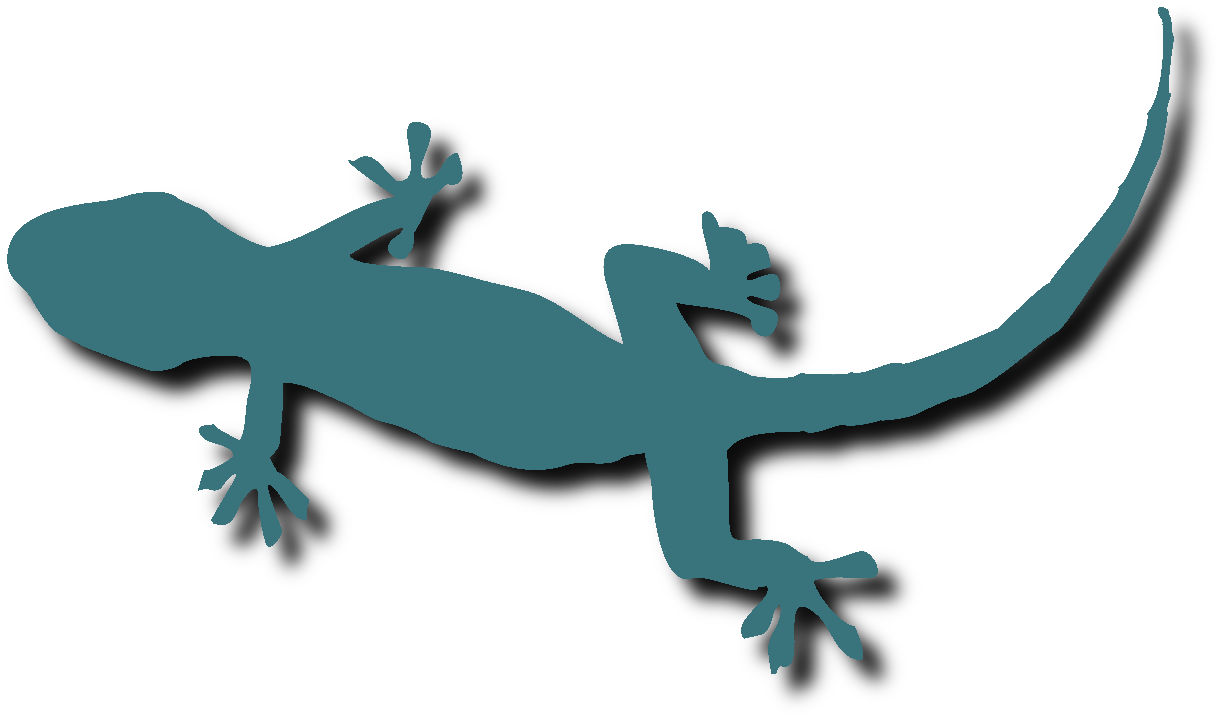
\includegraphics[width=15mm,resolution=150]{../images/phylopics/gecko-pixabay-cc0-5-teal-shadow.png}};
\node [visible on=<3>] at (n13h) {\hspace{20mm}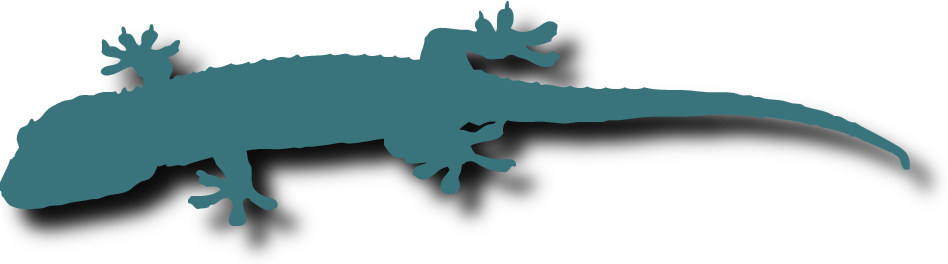
\includegraphics[width=15mm,resolution=150]{../images/phylopics/gekko-gecko-5-teal-shadow.png}};

\node [visible on=<4>] at (n3h) {\hspace{20mm}
\includegraphics[width=15mm,resolution=150]{../images/phylopics/gekko-vittatus-5-teal-shadow.png}};
\node [visible on=<4>] at (n6h) {\hspace{20mm}
\includegraphics[width=15mm,resolution=150]{../images/phylopics/gekko-vittatus-6-auburn-shadow.png}};
\node [visible on=<4>] at (n9h) {\hspace{20mm}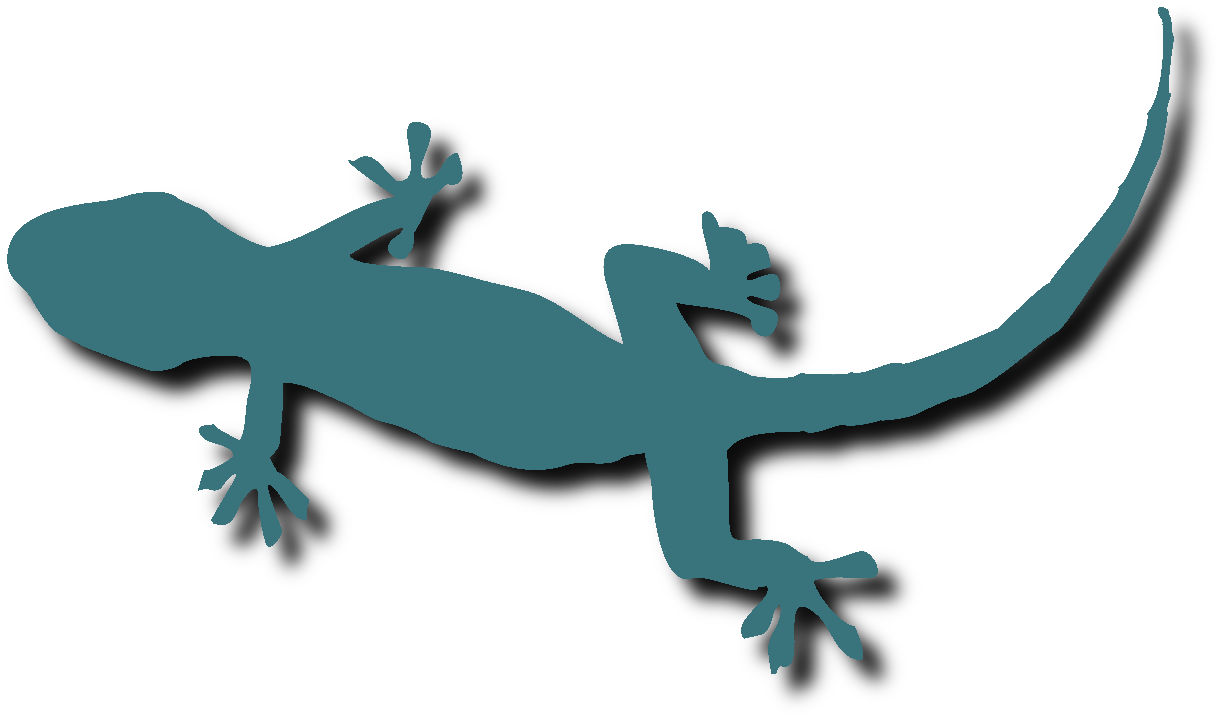
\includegraphics[width=15mm,resolution=150]{../images/phylopics/gecko-pixabay-cc0-5-teal-shadow.png}};
\node [visible on=<4>] at (n12h) {\hspace{20mm}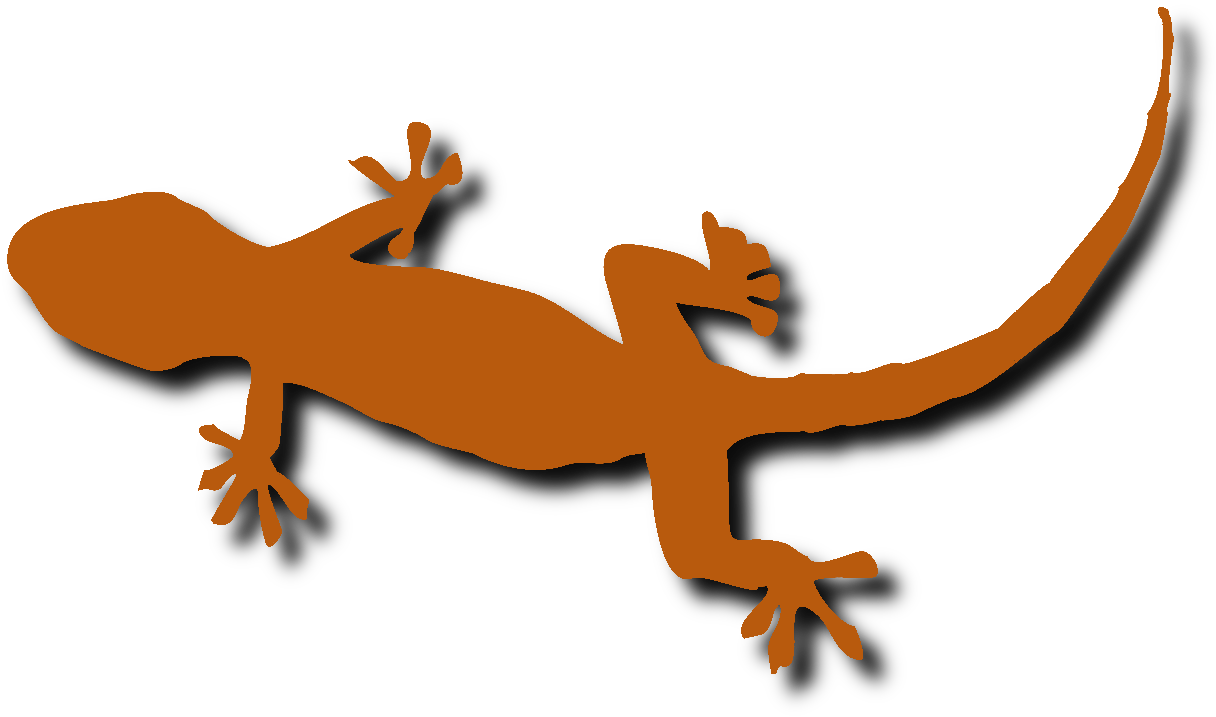
\includegraphics[width=15mm,resolution=150]{../images/phylopics/gecko-pixabay-cc0-6-auburn-shadow.png}};
\node [visible on=<4>] at (n14h) {\hspace{20mm}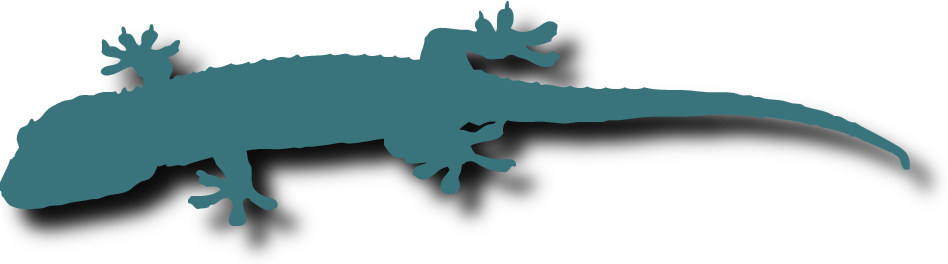
\includegraphics[width=15mm,resolution=150]{../images/phylopics/gekko-gecko-5-teal-shadow.png}};
\node [visible on=<4>] at (n17h) {\hspace{20mm}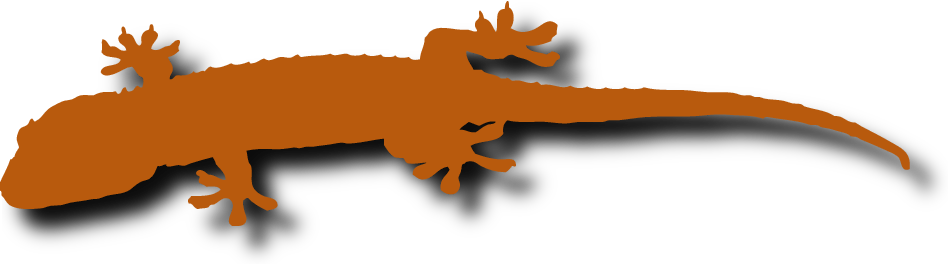
\includegraphics[width=15mm,resolution=150]{../images/phylopics/gekko-gecko-6-auburn-shadow.png}};

\node [visible on=<5->] at (n4) {\hspace{20mm}
\includegraphics[width=15mm,resolution=150]{../images/phylopics/gekko-vittatus-5-teal-shadow.png}};
\node [visible on=<5->] at (n5) {\hspace{20mm}\includegraphics[width=15mm,resolution=150]{../images/phylopics/gekko-vittatus-4-yellow-shadow.png}};
\node [visible on=<5->] at (n6) {\hspace{20mm}
\includegraphics[width=15mm,resolution=150]{../images/phylopics/gekko-vittatus-6-auburn-shadow.png}};
\node [visible on=<5->] at (n10) {\hspace{20mm}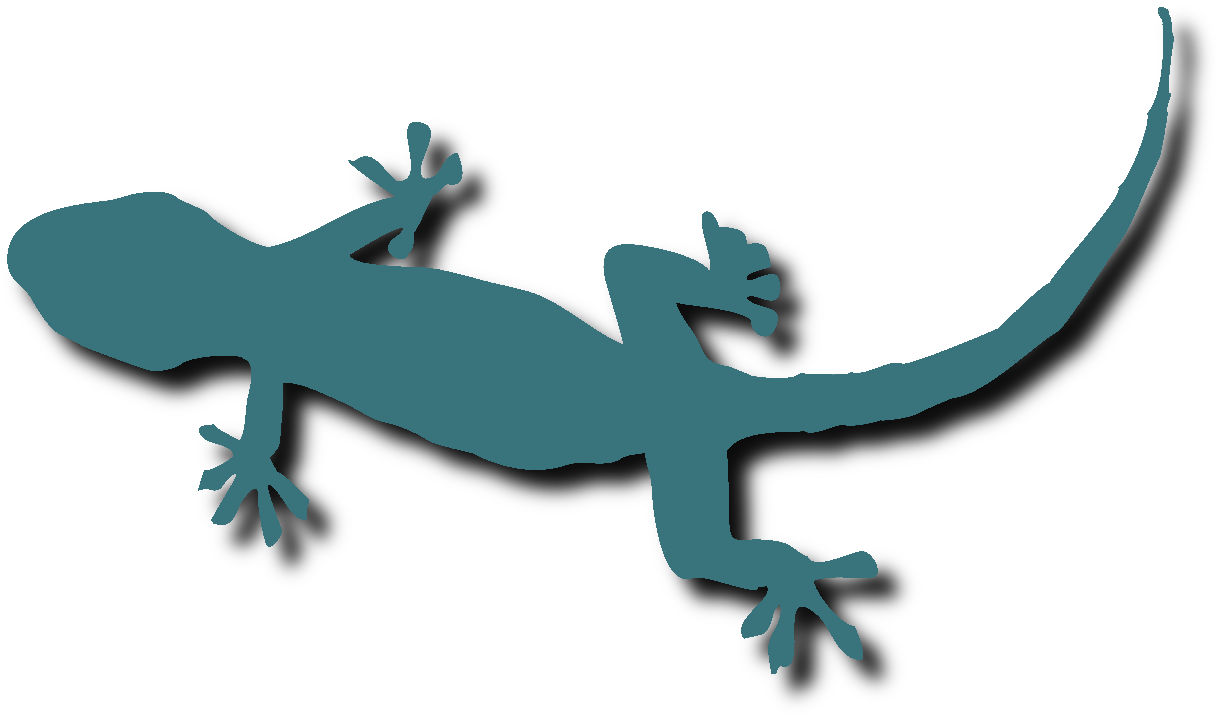
\includegraphics[width=15mm,resolution=150]{../images/phylopics/gecko-pixabay-cc0-5-teal-shadow.png}};
\node [visible on=<5->] at (n11) {\hspace{20mm}\includegraphics[width=15mm,resolution=150]{../images/phylopics/gecko-pixabay-cc0-4-yellow-shadow.png}};
\node [visible on=<5->] at (n12) {\hspace{20mm}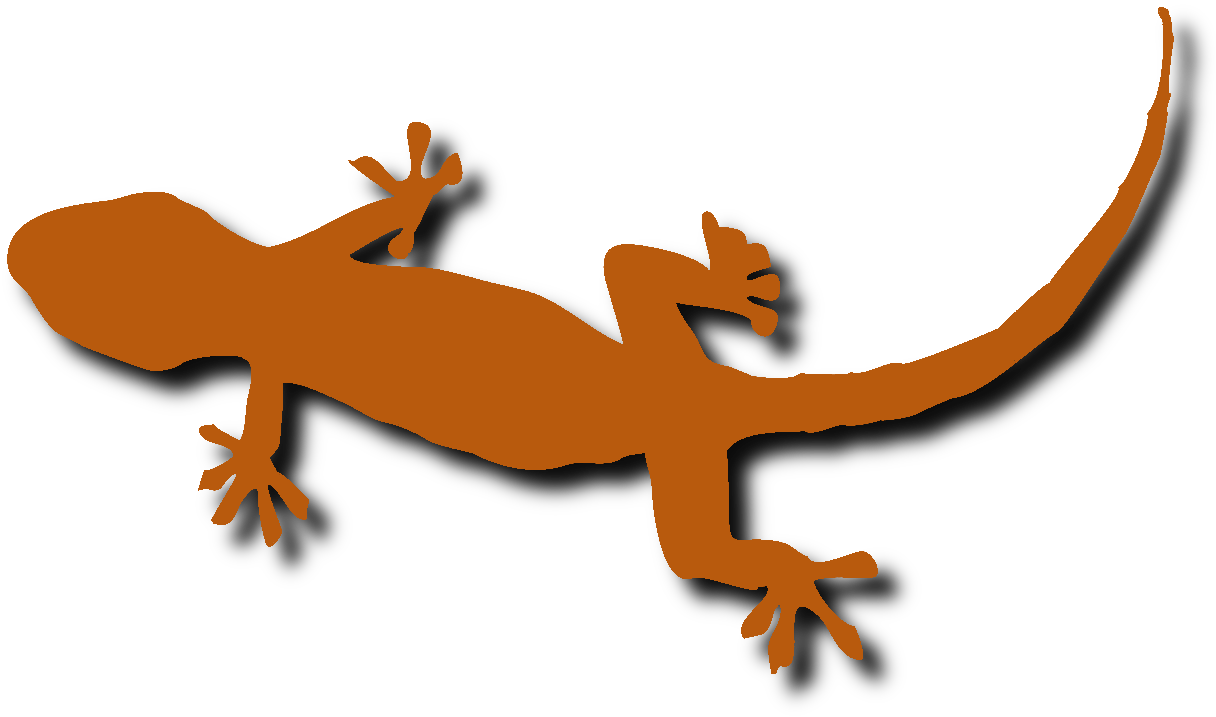
\includegraphics[width=15mm,resolution=150]{../images/phylopics/gecko-pixabay-cc0-6-auburn-shadow.png}};
\node [visible on=<5->] at (n15) {\hspace{20mm}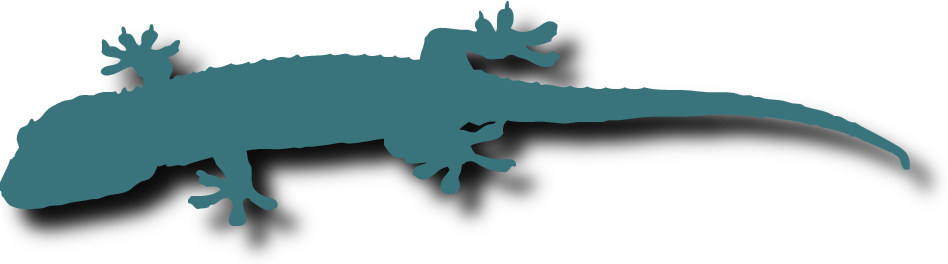
\includegraphics[width=15mm,resolution=150]{../images/phylopics/gekko-gecko-5-teal-shadow.png}};
\node [visible on=<5->] at (n16) {\hspace{20mm}\includegraphics[width=15mm,resolution=150]{../images/phylopics/gekko-gecko-4-yellow-shadow.png}};
\node [visible on=<5->] at (n17) {\hspace{20mm}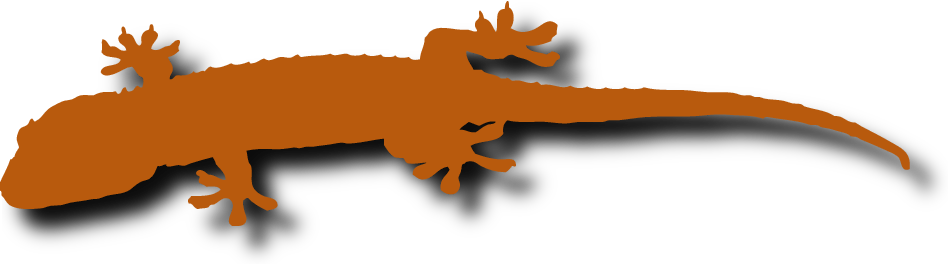
\includegraphics[width=15mm,resolution=150]{../images/phylopics/gekko-gecko-6-auburn-shadow.png}};

\end{tikzpicture}
}
}

\end{frame}

\begin{frame}[c]
    % \frametitle{Violating independent divergences}

%% This is a tikz file
\tikzset{node lower left/.style={font=\small,anchor=north east,text height=0.240cm,text depth=0.068cm,inner sep=0.03cm},
leaf/.style={font=\small,anchor=west,text height=0.240cm,text depth=0.068cm},
node upper left/.style={font=\small,anchor=south east,text height=0.240cm,text depth=0.068cm,inner sep=0.03cm},
bracket label/.style={font=\small,anchor=west,text height=0.240cm,text depth=0.068cm,inner sep=0.1cm},
node upper right/.style={font=\small,anchor=south west,text height=0.240cm,text depth=0.068cm,inner sep=0.03cm},
node right/.style={font=\small,anchor=west,text height=0.240cm,text depth=0.068cm,inner sep=0.03cm},
branch/.style={font=\tiny,text height=0.144cm,text depth=0.041cm,inner sep=0.025cm},
root/.style={font=\small,anchor=east,text height=0.240cm,text depth=0.068cm},
node lower right/.style={font=\small,anchor=north west,text height=0.240cm,text depth=0.068cm,inner sep=0.03cm}}

\centering{
\resizebox{!}{\frametextheight}{%
\begin{tikzpicture}[ultra thick,inner sep=0.1cm]
%  4:\hspace{20mm}\includegraphics[width=15mm]{../images/phylopics/gekko-vittatus-4-yellow-shadow.png}
%  3
% +2:\hspace{20mm}
\includegraphics[width=15mm]{../images/phylopics/gekko-vittatus-5-teal-shadow.png}
% ||
% |6:\hspace{20mm}
\includegraphics[width=15mm]{../images/phylopics/gekko-vittatus-6-auburn-shadow.png}
% |
% |10:\hspace{20mm}\includegraphics[width=15mm]{../images/phylopics/gecko-pixabay-cc0-4-yellow-shadow.png}
% 09
% |81:\hspace{20mm}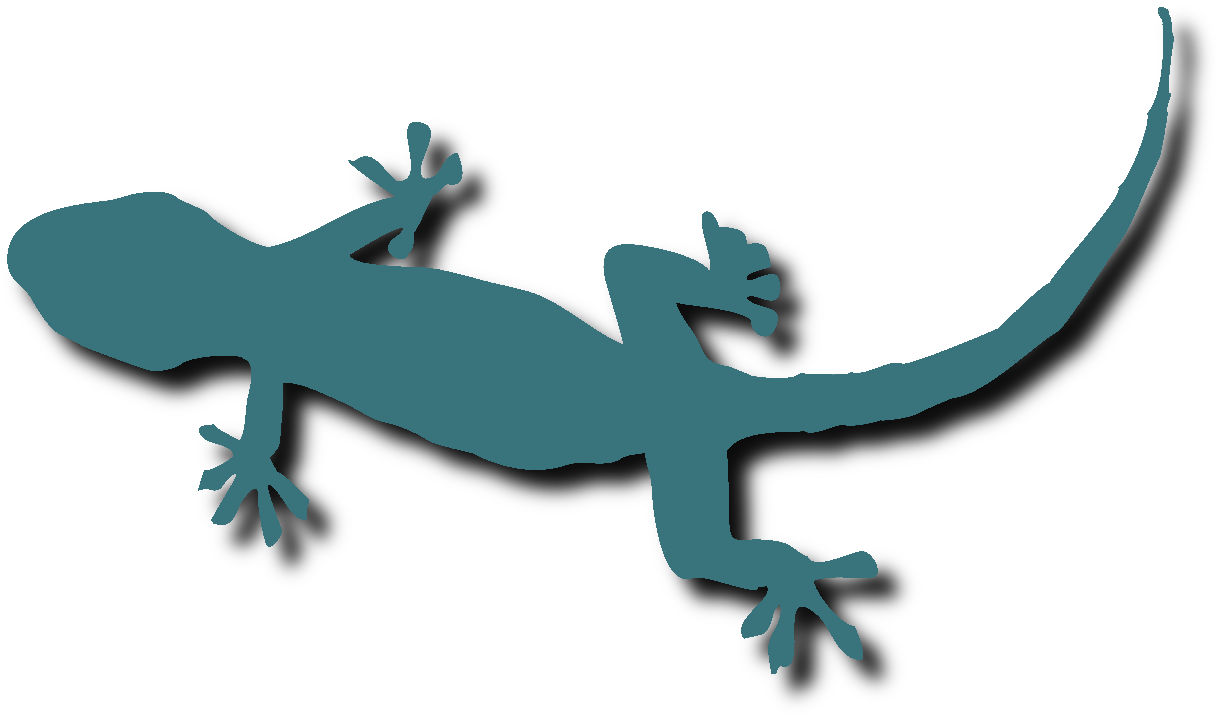
\includegraphics[width=15mm]{../images/phylopics/gecko-pixabay-cc0-5-teal-shadow.png}
% ||
% |12:\hspace{20mm}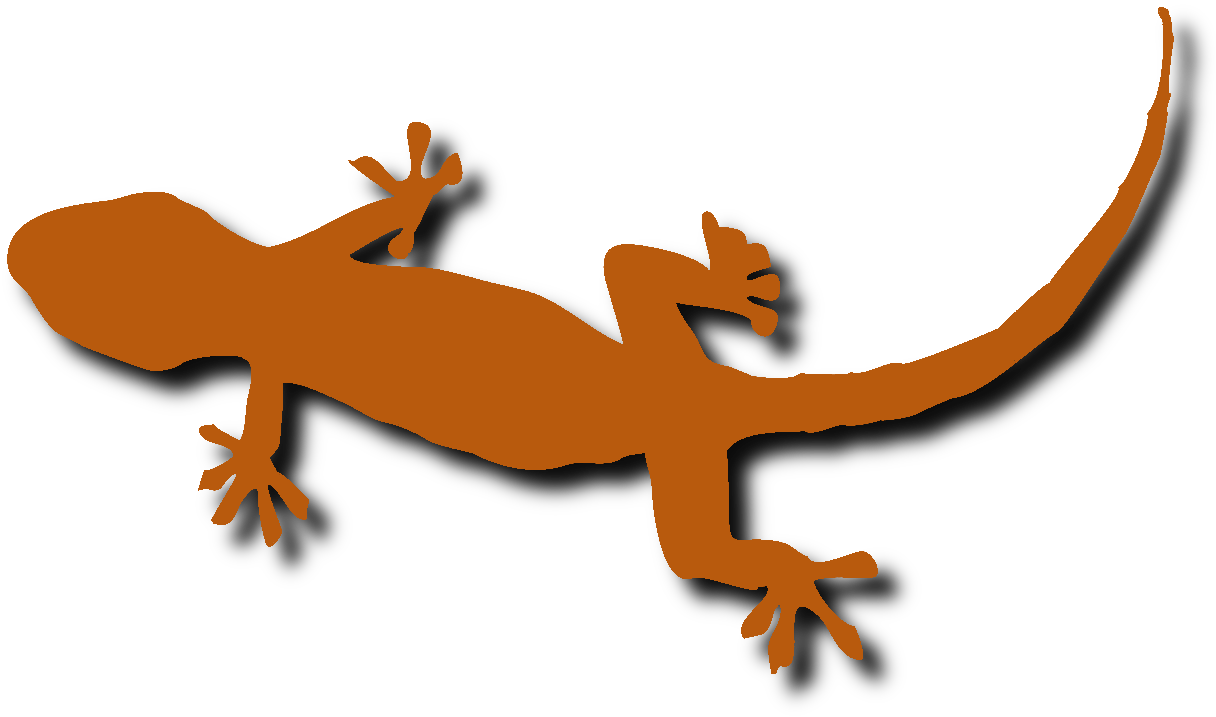
\includegraphics[width=15mm]{../images/phylopics/gecko-pixabay-cc0-6-auburn-shadow.png}
% 7
% |15:\hspace{20mm}\includegraphics[width=15mm]{../images/phylopics/gekko-gecko-4-yellow-shadow.png}
% |14
% +13:\hspace{20mm}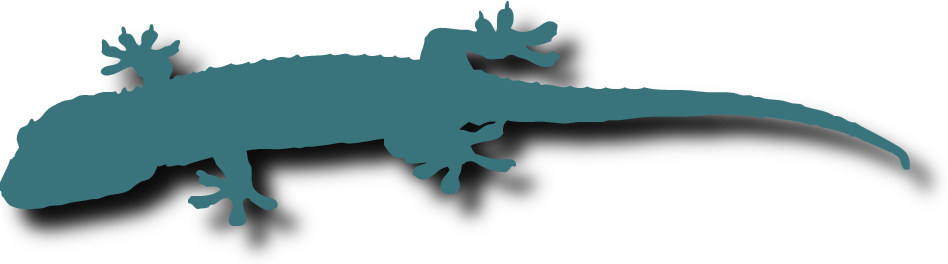
\includegraphics[width=15mm]{../images/phylopics/gekko-gecko-5-teal-shadow.png}
%  |
%  17:\hspace{20mm}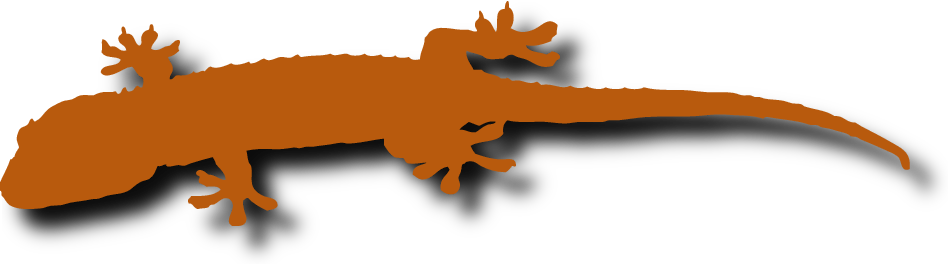
\includegraphics[width=15mm]{../images/phylopics/gekko-gecko-6-auburn-shadow.png}

% The scale is 1.000000, and the yScale is 0.800000

%% Coordinates of nodes.
\coordinate (island) at (11.6, 3.2);
\node[visible on=<1>] at (island) {\includegraphics[height=8.0cm]{../images/islands-1.pdf}};
\node[visible on=<2>] at (island) {\includegraphics[height=8.0cm]{../images/islands-2.pdf}};
\node[visible on=<3>] at (island) {\includegraphics[height=8.0cm]{../images/islands-3.pdf}};
\node[visible on=<4->] at (island) {\includegraphics[height=8.0cm]{../images/islands-3-bare.pdf}};

\draw [visible on=<3>, pteal,very thick,dashed] (6.600,-0.300) -- (6.600,6.728);
% \node [font=\LARGE,yshift=-0.200cm,text height=0.415cm,text depth=0.118cm] at (6.600,-0.300) {\color{pteal}$\tau_{\scriptscriptstyle 1}$};
\draw [visible on=<2->, pauburn,very thick,dashed] (4.600,-0.300) -- (4.600,6.728);
% \node [font=\LARGE,yshift=-0.200cm,text height=0.415cm,text depth=0.118cm] at (4.600,-0.300) {\color{pauburn}$\tau_{\scriptscriptstyle 2}$};
\coordinate (n0) at (0.000,3.600);
\coordinate (n1) at (0.100,3.600);
\coordinate (n1p) at (0.000,3.600);
\coordinate (n2) at (4.600,5.400);
\coordinate (n2h) at (3.200,5.400);
\coordinate (n2p) at (0.100,5.400);
\coordinate (n3) at (6.600,6.000);
\coordinate (n3p) at (4.600,6.000);
\coordinate (n3h) at (5.500,6.000);
\coordinate (n4) at (7.100,6.400);
\coordinate (n4p) at (6.600,6.400);
\coordinate (n4px) at (4.600,6.400);
\coordinate (n5) at (7.100,5.600);
\coordinate (n5p) at (6.600,5.600);
\coordinate (n5px) at (4.600,5.600);
\coordinate (n6) at (7.100,4.800);
\coordinate (n6p) at (4.600,4.800);
\coordinate (n6h) at (5.500,4.800);
\coordinate (n7) at (1.100,1.800);
\coordinate (n7p) at (0.100,1.800);
\coordinate (n8) at (4.600,3.000);
\coordinate (n8h) at (3.200,3.000);
\coordinate (n8p) at (1.100,3.000);
\coordinate (n9) at (6.600,3.600);
\coordinate (n9p) at (4.600,3.600);
\coordinate (n9h) at (5.500,3.600);
\coordinate (n10) at (7.100,4.000);
\coordinate (n10p) at (6.600,4.000);
\coordinate (n10px) at (4.600,4.000);
\coordinate (n11) at (7.100,3.200);
\coordinate (n11p) at (6.600,3.200);
\coordinate (n11px) at (4.600,3.200);
\coordinate (n12) at (7.100,2.400);
\coordinate (n12p) at (4.600,2.400);
\coordinate (n12h) at (5.500,2.400);
\coordinate (n13) at (4.600,0.600);
\coordinate (n13h) at (3.200,0.600);
\coordinate (n13p) at (1.100,0.600);
\coordinate (n14) at (6.600,1.200);
\coordinate (n14p) at (4.600,1.200);
\coordinate (n14h) at (5.500,1.200);
\coordinate (n15) at (7.100,1.600);
\coordinate (n15p) at (6.600,1.600);
\coordinate (n15px) at (4.600,1.600);
\coordinate (n16) at (7.100,0.800);
\coordinate (n16p) at (6.600,0.800);
\coordinate (n16px) at (4.600,0.800);
\coordinate (n17) at (7.100,0.000);
\coordinate (n17p) at (4.600,0.000);
\coordinate (n17h) at (5.500,0.000);

%% horizontal lines
\draw [visible on=<1->] (n1p) -- (n1);
\draw [visible on=<1>] (n2p) -- (n2h);
\draw [visible on=<2->] (n2p) -- (n2);
\draw [visible on=<3>] (n3p) -- (n3);
\draw [visible on=<2>] (n3p) -- (n3h);
\draw [visible on=<3>] (n4p) -- (n4);
\draw [visible on=<3>] (n5p) -- (n5);
\draw [visible on=<4->] (n4px) -- (n4);
\draw [visible on=<4->] (n5px) -- (n5);
\draw [visible on=<3->] (n6p) -- (n6);
\draw [visible on=<2>] (n6p) -- (n6h);
\draw [visible on=<1->] (n7p) -- (n7);
\draw [visible on=<1>] (n8p) -- (n8h);
\draw [visible on=<2->] (n8p) -- (n8);
\draw [visible on=<3>] (n9p) -- (n9);
\draw [visible on=<2>] (n9p) -- (n9h);
\draw [visible on=<3>] (n10p) -- (n10);
\draw [visible on=<3>] (n11p) -- (n11);
\draw [visible on=<4->] (n10px) -- (n10);
\draw [visible on=<4->] (n11px) -- (n11);
\draw [visible on=<3->] (n12p) -- (n12);
\draw [visible on=<2>] (n12p) -- (n12h);
\draw [visible on=<1>] (n13p) -- (n13h);
\draw [visible on=<2->] (n13p) -- (n13);
\draw [visible on=<3>] (n14p) -- (n14);
\draw [visible on=<2>] (n14p) -- (n14h);
\draw [visible on=<3>] (n15p) -- (n15);
\draw [visible on=<3>] (n16p) -- (n16);
\draw [visible on=<4->] (n15px) -- (n15);
\draw [visible on=<4->] (n16px) -- (n16);
\draw [visible on=<3->] (n17p) -- (n17);
\draw [visible on=<2>] (n17p) -- (n17h);

%% vertical lines
\draw [visible on=<1->,line cap=rect] (n2p) -- (n7p);
\draw [visible on=<2->,line cap=rect] (n3p) -- (n6p);
\draw [visible on=<3>,line cap=rect] (n4p) -- (n5p);
\draw [visible on=<4->,line cap=rect] (n4px) -- (n5px);
\draw [visible on=<1->,line cap=rect] (n8p) -- (n13p);
\draw [visible on=<2->,line cap=rect] (n9p) -- (n12p);
\draw [visible on=<3>,line cap=rect] (n10p) -- (n11p);
\draw [visible on=<4->,line cap=rect] (n10px) -- (n11px);
\draw [visible on=<2->,line cap=rect] (n14p) -- (n17p);
\draw [visible on=<3>,line cap=rect] (n15p) -- (n16p);
\draw [visible on=<4->,line cap=rect] (n15px) -- (n16px);

%% leaf labels
\node [visible on=<1>] at (n2h) {\hspace{20mm}\includegraphics[width=15mm]{../images/phylopics/gekko-vittatus-5-teal-shadow.png}};
\node [visible on=<1>] at (n8h) {\hspace{20mm}\includegraphics[width=15mm]{../images/phylopics/gecko-pixabay-cc0-5-teal-shadow.png}};
\node [visible on=<1>] at (n13h) {\hspace{20mm}\includegraphics[width=15mm]{../images/phylopics/gekko-gecko-5-teal-shadow.png}};

\node [visible on=<2>] at (n3h) {\hspace{20mm}\includegraphics[width=15mm]{../images/phylopics/gekko-vittatus-5-teal-shadow.png}};
\node [visible on=<2>] at (n6h) {\hspace{20mm}\includegraphics[width=15mm]{../images/phylopics/gekko-vittatus-6-auburn-shadow.png}};
\node [visible on=<2>] at (n9h) {\hspace{20mm}\includegraphics[width=15mm]{../images/phylopics/gecko-pixabay-cc0-5-teal-shadow.png}};
\node [visible on=<2>] at (n12h) {\hspace{20mm}\includegraphics[width=15mm]{../images/phylopics/gecko-pixabay-cc0-6-auburn-shadow.png}};
\node [visible on=<2>] at (n14h) {\hspace{20mm}\includegraphics[width=15mm]{../images/phylopics/gekko-gecko-5-teal-shadow.png}};
\node [visible on=<2>] at (n17h) {\hspace{20mm}\includegraphics[width=15mm]{../images/phylopics/gekko-gecko-6-auburn-shadow.png}};

\node [visible on=<3->] at (n4) {\hspace{20mm}\includegraphics[width=15mm]{../images/phylopics/gekko-vittatus-5-teal-shadow.png}};
\node [visible on=<3->] at (n5) {\hspace{20mm}\includegraphics[width=15mm]{../images/phylopics/gekko-vittatus-4-yellow-shadow.png}};
\node [visible on=<3->] at (n6) {\hspace{20mm}\includegraphics[width=15mm]{../images/phylopics/gekko-vittatus-6-auburn-shadow.png}};
\node [visible on=<3->] at (n10) {\hspace{20mm}\includegraphics[width=15mm]{../images/phylopics/gecko-pixabay-cc0-5-teal-shadow.png}};
\node [visible on=<3->] at (n11) {\hspace{20mm}\includegraphics[width=15mm]{../images/phylopics/gecko-pixabay-cc0-4-yellow-shadow.png}};
\node [visible on=<3->] at (n12) {\hspace{20mm}\includegraphics[width=15mm]{../images/phylopics/gecko-pixabay-cc0-6-auburn-shadow.png}};
\node [visible on=<3->] at (n15) {\hspace{20mm}\includegraphics[width=15mm]{../images/phylopics/gekko-gecko-5-teal-shadow.png}};
\node [visible on=<3->] at (n16) {\hspace{20mm}\includegraphics[width=15mm]{../images/phylopics/gekko-gecko-4-yellow-shadow.png}};
\node [visible on=<3->] at (n17) {\hspace{20mm}\includegraphics[width=15mm]{../images/phylopics/gekko-gecko-6-auburn-shadow.png}};

\end{tikzpicture}
}
}

\end{frame}


\begin{frame}[c,label=violations]
    % \frametitle{Violations are pervasive and interesting}
    % \frametitle{Shared divergences are pervasive and interesting}

    \begin{columns}

        \column{0.52\textwidth}

        \begin{minipage}[c][\frametextheight][c]{0.95\columnwidth}
            \raggedright
            \uncover<1->{
            Biogeography
            \begin{itemize}
                \item Environmental changes that affect whole communities of species
            \end{itemize}
            }

            \uncover<2->{
            Gene family evolution
            \begin{itemize}
                \item Chromosomal duplications
            \end{itemize}
            }

            \uncover<3->{
            Epidemiology
            \begin{itemize}
                \item Disease spread via co-infected individuals
                \item Transmission at social gatherings
            \end{itemize}
            }

            \uncover<4->{
            Endosymbiont evolution (e.g., parasites, microbiome)
            \begin{itemize}
                \item Speciation of the host
                \item Co-colonization of new host species
            \end{itemize}
            }
        \end{minipage}

        \column{0.46\textwidth}

        \begin{minipage}[c][\contentheight][c]{\columnwidth}
            \centering
            % \resizebox{!}{0.75\frametextheight}{%
            \resizebox{!}{0.71\frametextheight}{%
                \input{shared-div-tree.tex}
            }
        \end{minipage}
    \end{columns}

\end{frame}

\begin{frame}<handout:0|beamer:0>[noframenumbering,label=whycare]
    \frametitle{Why account for shared divergences?}

    \begin{enumerate}
        \item<2-> Improve inference
        \vspace{3mm}
        \item<3-> \textbf{Provide a framework for studying processes of
                co-diversification}
    \end{enumerate}

\end{frame}

\againframe<1-2>{whycare}

% \input{shared-div-advantages.tex}
\input{shared-div-advantages-bare.tex}

\againframe<2->{whycare}

\againframe<4->{violations}


\begin{frame}[c]
    % \frametitle{Violating independent divergences}

%% This is a tikz file
\tikzset{node lower left/.style={font=\small,anchor=north east,text height=0.240cm,text depth=0.068cm,inner sep=0.03cm},
leaf/.style={font=\small,anchor=west,text height=0.240cm,text depth=0.068cm},
node upper left/.style={font=\small,anchor=south east,text height=0.240cm,text depth=0.068cm,inner sep=0.03cm},
bracket label/.style={font=\small,anchor=west,text height=0.240cm,text depth=0.068cm,inner sep=0.1cm},
node upper right/.style={font=\small,anchor=south west,text height=0.240cm,text depth=0.068cm,inner sep=0.03cm},
node right/.style={font=\small,anchor=west,text height=0.240cm,text depth=0.068cm,inner sep=0.03cm},
branch/.style={font=\tiny,text height=0.144cm,text depth=0.041cm,inner sep=0.025cm},
root/.style={font=\small,anchor=east,text height=0.240cm,text depth=0.068cm},
node lower right/.style={font=\small,anchor=north west,text height=0.240cm,text depth=0.068cm,inner sep=0.03cm}}

\centering{
\resizebox{!}{\frametextheight}{%
\begin{tikzpicture}[ultra thick,inner sep=0.1cm]
%  4:\hspace{20mm}\includegraphics[width=15mm]{../images/phylopics/gekko-vittatus-4-yellow-shadow.png}
%  3
% +2:\hspace{20mm}\includegraphics[width=15mm]{../images/phylopics/gekko-vittatus-5-teal-shadow.png}
% ||
% |6:\hspace{20mm}\includegraphics[width=15mm]{../images/phylopics/gekko-vittatus-6-auburn-shadow.png}
% |
% |10:\hspace{20mm}\includegraphics[width=15mm]{../images/phylopics/gecko-pixabay-cc0-4-yellow-shadow.png}
% 09
% |81:\hspace{20mm}\includegraphics[width=15mm]{../images/phylopics/gecko-pixabay-cc0-5-teal-shadow.png}
% ||
% |12:\hspace{20mm}\includegraphics[width=15mm]{../images/phylopics/gecko-pixabay-cc0-6-auburn-shadow.png}
% 7
% |15:\hspace{20mm}\includegraphics[width=15mm]{../images/phylopics/gekko-gecko-4-yellow-shadow.png}
% |14
% +13:\hspace{20mm}\includegraphics[width=15mm]{../images/phylopics/gekko-gecko-5-teal-shadow.png}
%  |
%  17:\hspace{20mm}\includegraphics[width=15mm]{../images/phylopics/gekko-gecko-6-auburn-shadow.png}

% The scale is 1.000000, and the yScale is 0.800000

%% Coordinates of nodes.
\coordinate (island) at (11.6, 3.2);
\node[visible on=<1>] at (island) {\includegraphics[height=8.0cm]{../images/island-cartoons/islands-1.pdf}};
\node[visible on=<2>] at (island) {\includegraphics[height=8.0cm]{../images/island-cartoons/islands-2.pdf}};
% \node[visible on=<3->] at (island) {\includegraphics[height=8.0cm,resolution=300]{../images/island-cartoons/islands-3.pdf}};

% \draw [visible on=<3->, pteal,very thick,dashed] (6.600,-0.300) -- (6.600,6.728);
% \node [font=\LARGE,yshift=-0.200cm,text height=0.415cm,text depth=0.118cm] at (6.600,-0.300) {\color{pteal}$\tau_{\scriptscriptstyle 1}$};
\draw [visible on=<2->, pauburn,very thick,dashed] (4.600,-0.300) -- (4.600,6.728);
% \node [font=\LARGE,yshift=-0.200cm,text height=0.415cm,text depth=0.118cm] at (4.600,-0.300) {\color{pauburn}$\tau_{\scriptscriptstyle 2}$};
\coordinate (n0) at (0.000,3.600);
\coordinate (n1) at (0.100,3.600);
\coordinate (n1p) at (0.000,3.600);
\coordinate (n2) at (4.600,5.400);
\coordinate (n2h) at (3.200,5.400);
\coordinate (n2p) at (0.100,5.400);
\coordinate (n3) at (6.600,6.000);
\coordinate (n3p) at (4.600,6.000);
\coordinate (n3h) at (5.500,6.000);
\coordinate (n4) at (7.100,6.400);
\coordinate (n4p) at (6.600,6.400);
\coordinate (n5) at (7.100,5.600);
\coordinate (n5p) at (6.600,5.600);
\coordinate (n6) at (7.100,4.800);
\coordinate (n6p) at (4.600,4.800);
\coordinate (n6h) at (5.500,4.800);
\coordinate (n7) at (1.100,1.800);
\coordinate (n7p) at (0.100,1.800);
\coordinate (n8) at (4.600,3.000);
\coordinate (n8h) at (3.200,3.000);
\coordinate (n8p) at (1.100,3.000);
\coordinate (n9) at (6.600,3.600);
\coordinate (n9p) at (4.600,3.600);
\coordinate (n9h) at (5.500,3.600);
\coordinate (n10) at (7.100,4.000);
\coordinate (n10p) at (6.600,4.000);
\coordinate (n11) at (7.100,3.200);
\coordinate (n11p) at (6.600,3.200);
\coordinate (n12) at (7.100,2.400);
\coordinate (n12p) at (4.600,2.400);
\coordinate (n12h) at (5.500,2.400);
\coordinate (n13) at (4.600,0.600);
\coordinate (n13h) at (3.200,0.600);
\coordinate (n13p) at (1.100,0.600);
\coordinate (n14) at (6.600,1.200);
\coordinate (n14p) at (4.600,1.200);
\coordinate (n14h) at (5.500,1.200);
\coordinate (n15) at (7.100,1.600);
\coordinate (n15p) at (6.600,1.600);
\coordinate (n16) at (7.100,0.800);
\coordinate (n16p) at (6.600,0.800);
\coordinate (n17) at (7.100,0.000);
\coordinate (n17p) at (4.600,0.000);
\coordinate (n17h) at (5.500,0.000);

%% horizontal lines
\draw [visible on=<1->] (n1p) -- (n1);
\draw [visible on=<1>] (n2p) -- (n2h);
\draw [visible on=<2->] (n2p) -- (n2);
% \draw [visible on=<3->] (n3p) -- (n3);
\draw [visible on=<2>] (n3p) -- (n3h);
% \draw [visible on=<3->] (n4p) -- (n4);
% \draw [visible on=<3->] (n5p) -- (n5);
% \draw [visible on=<3->] (n6p) -- (n6);
\draw [visible on=<2>] (n6p) -- (n6h);
\draw [visible on=<1->] (n7p) -- (n7);
\draw [visible on=<1>] (n8p) -- (n8h);
\draw [visible on=<2->] (n8p) -- (n8);
% \draw [visible on=<3->] (n9p) -- (n9);
\draw [visible on=<2>] (n9p) -- (n9h);
% \draw [visible on=<3->] (n10p) -- (n10);
% \draw [visible on=<3->] (n11p) -- (n11);
% \draw [visible on=<3->] (n12p) -- (n12);
\draw [visible on=<2>] (n12p) -- (n12h);
\draw [visible on=<1>] (n13p) -- (n13h);
\draw [visible on=<2->] (n13p) -- (n13);
% \draw [visible on=<3->] (n14p) -- (n14);
\draw [visible on=<2>] (n14p) -- (n14h);
% \draw [visible on=<3->] (n15p) -- (n15);
% \draw [visible on=<3->] (n16p) -- (n16);
% \draw [visible on=<3->] (n17p) -- (n17);
\draw [visible on=<2>] (n17p) -- (n17h);

%% vertical lines
\draw [visible on=<1->,line cap=rect] (n2p) -- (n7p);
\draw [visible on=<2->,line cap=rect] (n3p) -- (n6p);
% \draw [visible on=<3->,line cap=rect] (n4p) -- (n5p);
\draw [visible on=<1->,line cap=rect] (n8p) -- (n13p);
\draw [visible on=<2->,line cap=rect] (n9p) -- (n12p);
% \draw [visible on=<3->,line cap=rect] (n10p) -- (n11p);
\draw [visible on=<2->,line cap=rect] (n14p) -- (n17p);
% \draw [visible on=<3->,line cap=rect] (n15p) -- (n16p);

%% leaf labels
\node [visible on=<1>] at (n2h) {\hspace{20mm}\includegraphics[width=15mm]{../images/phylopics/gekko-vittatus-5-teal-shadow.png}};
\node [visible on=<1>] at (n8h) {\hspace{20mm}\includegraphics[width=15mm]{../images/phylopics/gecko-pixabay-cc0-5-teal-shadow.png}};
\node [visible on=<1>] at (n13h) {\hspace{20mm}\includegraphics[width=15mm]{../images/phylopics/gekko-gecko-5-teal-shadow.png}};

\node [visible on=<2>] at (n3h) {\hspace{20mm}\includegraphics[width=15mm]{../images/phylopics/gekko-vittatus-5-teal-shadow.png}};
\node [visible on=<2>] at (n6h) {\hspace{20mm}\includegraphics[width=15mm]{../images/phylopics/gekko-vittatus-6-auburn-shadow.png}};
\node [visible on=<2>] at (n9h) {\hspace{20mm}\includegraphics[width=15mm]{../images/phylopics/gecko-pixabay-cc0-5-teal-shadow.png}};
\node [visible on=<2>] at (n12h) {\hspace{20mm}\includegraphics[width=15mm]{../images/phylopics/gecko-pixabay-cc0-6-auburn-shadow.png}};
\node [visible on=<2>] at (n14h) {\hspace{20mm}\includegraphics[width=15mm]{../images/phylopics/gekko-gecko-5-teal-shadow.png}};
\node [visible on=<2>] at (n17h) {\hspace{20mm}\includegraphics[width=15mm]{../images/phylopics/gekko-gecko-6-auburn-shadow.png}};

% \node [visible on=<3->] at (n4) {\hspace{20mm}\includegraphics[width=15mm]{../images/phylopics/gekko-vittatus-5-teal-shadow.png}};
% \node [visible on=<3->] at (n5) {\hspace{20mm}\includegraphics[width=15mm]{../images/phylopics/gekko-vittatus-4-yellow-shadow.png}};
% \node [visible on=<3->] at (n6) {\hspace{20mm}\includegraphics[width=15mm]{../images/phylopics/gekko-vittatus-6-auburn-shadow.png}};
% \node [visible on=<3->] at (n10) {\hspace{20mm}\includegraphics[width=15mm]{../images/phylopics/gecko-pixabay-cc0-5-teal-shadow.png}};
% \node [visible on=<3->] at (n11) {\hspace{20mm}\includegraphics[width=15mm]{../images/phylopics/gecko-pixabay-cc0-4-yellow-shadow.png}};
% \node [visible on=<3->] at (n12) {\hspace{20mm}\includegraphics[width=15mm]{../images/phylopics/gecko-pixabay-cc0-6-auburn-shadow.png}};
% \node [visible on=<3->] at (n15) {\hspace{20mm}\includegraphics[width=15mm]{../images/phylopics/gekko-gecko-5-teal-shadow.png}};
% \node [visible on=<3->] at (n16) {\hspace{20mm}\includegraphics[width=15mm]{../images/phylopics/gekko-gecko-4-yellow-shadow.png}};
% \node [visible on=<3->] at (n17) {\hspace{20mm}\includegraphics[width=15mm]{../images/phylopics/gekko-gecko-6-auburn-shadow.png}};

\end{tikzpicture}
}
}

\end{frame}


\begin{frame}[t]
    % \frametitle<1->{Divergence model choice}

    \begin{center}
    \smartgraphic{<1>}{../images/from-ecoevolity-tikz-repo/div-model-111-labels.pdf}

    \smartgraphic{<2>}{../images/from-ecoevolity-tikz-repo/div-model-311-labels.pdf}

    \smartgraphic{<3>}{../images/from-ecoevolity-tikz-repo/div-model-131-labels.pdf}

    \smartgraphic{<4>}{../images/from-ecoevolity-tikz-repo/div-model-113-labels.pdf}

    \smartgraphic{<5>}{../images/from-ecoevolity-tikz-repo/div-model-213-labels.pdf}
    \end{center}
\end{frame}


    
\begin{frame}[t,label=fullmodel]
    % \frametitle{Divergence-model choice}
    % \frametitle{Inferring co-diversification}

    % \vspace{-3.5mm}

    \begin{minipage}[t][0.35\textheight][t]{\linewidth}
        \centerline{
            \only<1-2>{
            \begin{tabu} to 1.05\linewidth { X[c] X[c] X[c] X[c] X[c] }
                $\divModel{1}$ & 
                $\divModel{2}$ & 
                $\divModel{3}$ & 
                $\divModel{4}$ & 
                $\divModel{5}$ \\
            \end{tabu}
            }
            \only<3->{
            \hspace{-4mm}
            \begin{tabu} to 1.05\linewidth { X[c] X[c] X[c] X[c] X[c] }
                $p(\divModel{1} \given \alignmentVector)$ & 
                $p(\divModel{2} \given \alignmentVector)$ & 
                $p(\divModel{3} \given \alignmentVector)$ & 
                $p(\divModel{4} \given \alignmentVector)$ & 
                $p(\divModel{5} \given \alignmentVector)$ \\
            \end{tabu}
            }
        }
        % \hspace{0mm}

        \centerline{
        \includegraphics<1->[width=0.18\linewidth]{../images/from-ecoevolity-tikz-repo/div-model-111-lines-small.pdf}
        % \hspace{12.0mm}
        \hspace{1.3mm}
        \includegraphics<1->[width=0.18\linewidth]{../images/from-ecoevolity-tikz-repo/div-model-311-lines-small.pdf}
        % \hspace{5.6mm}
        \hspace{1.3mm}
        \includegraphics<1->[width=0.18\linewidth]{../images/from-ecoevolity-tikz-repo/div-model-131-lines-small.pdf}
        % \hspace{5.6mm}
        \hspace{1.3mm}
        \includegraphics<1->[width=0.18\linewidth]{../images/from-ecoevolity-tikz-repo/div-model-113-lines-small.pdf}
        % \hspace{5.6mm}
        \hspace{1.3mm}
        \includegraphics<1->[width=0.18\linewidth]{../images/from-ecoevolity-tikz-repo/div-model-213-lines-small.pdf}
        }
    \end{minipage}

    \vspace{-1mm}

    \begin{minipage}[t][0.45\textheight][t]{\linewidth}
        \begin{onlyenv}<2-6>
            \begin{center}
                We want to infer the model and divergence times given genetic data
            \end{center}
        \end{onlyenv}

        \vspace{-3mm}
        \begin{onlyenv}<4-6>
            \begin{displaybox}[0.60\linewidth]
                \vspace{-1.3mm}
                \only<4-6>{
                    \[
                        p(\divModel{i} \given \alignmentVector) \propto
                        % \frac{
                            p(\alignmentVector \given \divModel{i})
                            p(\divModel{i})
                        % }{
                            % \sum_{i} p(\alignmentVector \given \divModel{i})
                            % p(\divModel{i})
                        % }
                    \]\vspace{0mm}
                }

                \vspace{-5mm}

            \end{displaybox}
        \end{onlyenv}

        \vspace{0.5mm}
        \begin{onlyenv}<5-6>
            \begin{displaybox}[0.60\linewidth]
                \vspace{-4.1mm}
                \only<5-6>{
                    \[
                        p(\alignmentVector \given \divModel{i}) = 
                        \int_{\allParameters{}}
                        p(\alignmentVector \given \allParameters{}, \divModel{i})
                        p(\allParameters{} \given \divModel{i})
                        d\allParameters{}
                    \]%\vspace{1mm}
                }

                %\vspace{-4mm}

            \end{displaybox}
        \end{onlyenv}

        \vspace{-1.5mm}
        \begin{onlyenv}<6>
            \begin{columns}

                \column{0.42\linewidth}

                \begin{itemize}
                    \small
                    \item Divergence times
                    \item Gene trees
                \end{itemize}

                \column{0.42\linewidth}

                \begin{itemize}
                    \small
                    \item Substitution parameters
                    \item Demographic parameters
                \end{itemize}
            \end{columns}
        \end{onlyenv}
        
        \begin{onlyenv}<7->
            \vspace{3.0mm}
            \textbf{Challenges:} \\
            \vspace{-6mm}
            \begin{enumerate}
                % \item<8-> Cannot solve all the integrals analytically
                \item<8-> Likelihood is tractable, but difficult 
                % \begin{itemize}
                %     \item<10-> Numerical approximation via approximate-likelihood Bayesian computation (ABC)
                % \end{itemize}
                \item<9-> Sampling over all possible models
                \begin{itemize}
                    \item<10-> 5 taxa = 52 models
                    \item<11-> 10 taxa = 115,975 models
                    \item<12-> 20 taxa = 51,724,158,235,372 models!!
                    % \item<15-> A ``diffuse'' Dirichlet process prior (DPP)
                \end{itemize}
            \end{enumerate}
        \end{onlyenv}
    \end{minipage}
    \vspace{-0.5cm}
    % \barefootnote{\tiny \shortfullcite{Oaks2012}, \shortfullcite{Oaks2014dpp}}
\end{frame}



\begin{frame}

    \begin{itemize}
        \item<1-> Let's assume we are interested in the probability of a coin we
            have not seen landing heads-side up when it is flipped
            (\probheads)

        \item<2-> Before flipping, we decide to compare two models that vary in our
            prior assumptions about the probability of the coin landing heads
            up

        \item<3-> We assume:
        \begin{enumerate}
            \item The coin is probably fair \\

                \vspace{1.0ex}
                \coinmodel[1]: $\probheads \sim \textrm{Beta}(5.0, 5.0)$

            \vspace{2ex}
            \item the coin is weighted to land tails side up most of time \\

                \vspace{1.0ex}
                \coinmodel[2]: $\probheads \sim \textrm{Beta}(1.0, 5.0)$
        \end{enumerate}
    \end{itemize}
\end{frame}


\begin{frame}
    \begin{itemize}
        \item<1-> We do 100 flips and 50 land heads up

        \item<2-> Now, we can calculate the posterior distribution for
            the probability of landing heads up under both our models
    \end{itemize}

    \onslide<3->{
    \begin{displaybox}[0.60\linewidth]
        \[
            p(\probheads \given \flipdata, \coinmodel[i]) = \frac{
                p(\flipdata \given \probheads, \coinmodel[i]) p(\probheads \given \coinmodel[i])
            }{
                p(\flipdata \given \coinmodel[i])
            }
        \]
    \end{displaybox}
    }

    \begin{itemize}
        \item<4-> We see the posterior distribution of \probheads is very
            robust to our prior assumptions

        \item<4-> \href{https://kerrycobb.github.io/beta-binomial-web-demo/}{https://kerrycobb.github.io/beta-binomial-web-demo/}
    \end{itemize}
\end{frame}


\begin{frame}
    \begin{itemize}
        \item<1-> However, we want to compare the ability of the models to explain the
            data
        \item<2-> We need to average (integrate) the likelihood density function
            over all possible values of \probheads, weighting by the prior
    \end{itemize}

    \onslide<3->{
    \begin{displaybox}[0.60\linewidth]
        \vspace{-2ex}
        \[
            p(\flipdata \given \coinmodel[1]) =
            \int_{\probheads}
            p( \flipdata \given \probheads, \coinmodel[1])
            p(\probheads \given \coinmodel[1])
            \diff{\probheads}
        \]
    \end{displaybox}
    }
\end{frame}


\begin{frame}
    \begin{itemize}
        \item<1-> Why do we care about the marginal likelihood?
        \item<2-> It's \emph{the evidence} that updates our prior to give us
            the posterior probability of the model
    \end{itemize}

    \onslide<3->{
    \begin{displaybox}[0.80\linewidth]
        \vspace{0.7ex}
        \[
            p(\coinmodel[1] \given \flipdata) = \frac{
                p(\flipdata \given \coinmodel[1])
                p(\coinmodel[1])
            }{
                p(\flipdata \given \coinmodel[1])
                p(\coinmodel[1])
                +
                p(\flipdata \given \coinmodel[2])
                p(\coinmodel[2])
            }
        \]
        \vspace{0ex}
    \end{displaybox}
    }
\end{frame}


\againframe<7->{fullmodel}

\begin{frame}
    \begin{center}
        \LARGE
        \href{https://github.com/phyletica/ecoevolity}{
            \textbf{\textcolor{pgreen}{E}\textcolor{pteal}{co\textcolor{pauburn}{evo}lity}}}:
        \textcolor{pgreen}{\bf E}stimating \textcolor{pauburn}{\bf evo}lutionary \textcolor{pteal}{\bf coevality}
    \end{center}

    \begin{itemize}
        \item<2-> CTMC model of characters evolving along genealogies
        \item<2-> Coalescent model of genealogies branching within populations
        \item<2-> Dirichlet-process prior across divergence models
        \item<2-> Gibbs sampling\footnote{\tiny\shortfullcite{Neal2000}}
                  to numerically sample models
        \item<2-> Analytically integrate over genealogies\footnote{\tiny\shortfullcite{Bryant2012}}

        \bigskip
        \item<3-> \textsl{Goal: Fast, full-likelihood Bayesian method to infer
                patterns of co-diversification from genome-scale data}
    \end{itemize}
\end{frame}


% \input{paic-study.tex}

% \begin{frame}[t,label=challenges]
    \frametitle{Approach \#1}

    \textbf{Challenges:} \\
    \begin{minipage}[t][0.35\textheight][t]{\linewidth}
    \begin{enumerate}
        % \item<8-> Cannot solve all the integrals analytically
        \item<1-> Likelihood is tractable, but difficult
        \begin{itemize}
            \item<2-> Use an existing method!
        \end{itemize}
        % \begin{itemize}
        %     \item<2-> Numerical approximation via approximate-likelihood Bayesian computation (ABC)
        % \end{itemize}
    \end{enumerate}
    \end{minipage}

    \begin{minipage}[t][0.35\textheight][t]{\linewidth}
    \begin{enumerate}
        \setcounter{enumi}{1}
        \item<1-> Sampling over all possible models
        \begin{itemize}
            % \item<3-> A ``diffuse'' Dirichlet process prior (DPP)
            \item<2-> Use an existing method! 
        \end{itemize}
    \end{enumerate}
    \end{minipage}
    % \barefootnote{\tiny \shortfullcite{Oaks2012}, \shortfullcite{Oaks2014dpp}}
\end{frame}


% \begin{frame}[t]
    \vspace{-5mm}
    \begin{center}
    \smartgraphic{<1>}{../images/old-paic-results/negros-panay-msbayes.pdf}
    \end{center}
    \barefootnote{\shortfullcite{Oaks2012}}
\end{frame}


% \begin{frame}<handout:0|beamer:0>[t,noframenumbering,label=approach2]
    \frametitle{Approach \#2}

    \textbf{Challenges:} \\
    \begin{minipage}[t][0.35\textheight][t]{\linewidth}
    \begin{enumerate}
        % \item<8-> Cannot solve all the integrals analytically
        \item<1-> Likelihood is tractable, but difficult
        % \begin{itemize}
        %     \item<2-> Use an existing method!
        % \end{itemize}
        \begin{itemize}
            \item<2-> Numerical approximation via approximate-likelihood Bayesian computation (ABC)
        \end{itemize}
    \end{enumerate}
    \end{minipage}

    \begin{minipage}[t][0.35\textheight][t]{\linewidth}
    \begin{enumerate}
        \setcounter{enumi}{1}
        \item<1-> Sampling over all possible models
        \begin{itemize}
            \item<3-> A ``diffuse'' Dirichlet process prior (DPP)
            % \item<2-> Use an existing method! 
        \end{itemize}
    \end{enumerate}
    \end{minipage}
    % \barefootnote{\tiny \shortfullcite{Oaks2012}, \shortfullcite{Oaks2014dpp}}
\end{frame}

\againframe<1-2>{approach2}

\blankslide

\againframe<2->{approach2}


% \begin{frame}
\setbeamercovered{invisible}

% Set the overall layout of the tree
\tikzstyle{level 1}=[level distance=8em, sibling distance=10.8em]
\tikzstyle{level 2}=[level distance=11em, sibling distance=4.3em]

% Define styles
\tikzstyle{root} = [minimum width=12mm, minimum height=8mm]
\tikzstyle{internal} = [minimum width=12mm, minimum height=8mm]
\tikzstyle{tip} = [minimum width=12mm, minimum height=8mm]
\tikzstyle{branch} = [->, very thick]

\vspace{-2mm}
\uncover<6->{
\hspace{0.43\textwidth}
    {\LARGE $\boldsymbol{\alpha =} \only<6>{\mathbf{\conc}}\only<7->{\mathbf{\cconc}}$} \\
}

\vspace{4mm}

\hspace{1.2cm}
% \resizebox{!}{1.02\frametextheight}{%
\resizebox{!}{0.98\frametextheight}{%
\begin{tikzpicture}[grow=right]%, sloped]
\pgfkeys{/pgf/number format/.cd,fixed,fixed zerofill,precision=3}
\node[root] {\pgftext{\includegraphics[width=8mm]{../images/dpp-nodes/dpp-node-1.pdf}}}
    child [visible on=<2->]{
        node[internal] {\pgftext{\includegraphics[width=8mm]{../images/dpp-nodes/dpp-node-12.pdf}}}        
            child [visible on=<4->]{
                node[tip, label=right:
                    {\tiplabel{\uncover<5->{
                        $
                        % p(m = 123)=
                        \left(\frac{\alpha}{\alpha+1}\right)\left(\frac{\alpha}{\alpha+2}\right)
                        \only<6>{= \calcprob{\conc}{\conc}}
                        \uncover<7->{= \ccalcprob{\cconc}{\cconc}}$
                        }}}]
                    {\pgftext{\includegraphics[width=8mm]{../images/dpp-nodes/dpp-node-123.pdf}}}
                edge from parent [style = branch]
                node[above,
                    label={[label distance = -0.7em]\branchlabel{$\alpha$}}%$\frac{\alpha}}{\alpha+2}$}}
                    ] {}
            }
            child [visible on=<4->]{
                node[tip, label=right:
                    {\tiplabel{\uncover<5->{
                        $
                        % p(m = 121)=
                        \left(\frac{\alpha}{\alpha+1}\right)\left(\frac{1}{\alpha+2}\right)
                        \only<6>{= \calcprob{\conc}{1}}
                        \uncover<7->{= \ccalcprob{\cconc}{1}}$
                        }}}]
                    {\pgftext{\includegraphics[width=8mm]{../images/dpp-nodes/dpp-node-122.pdf}}}
                edge from parent [style = branch]
                node[above,
                    label={[label distance = -0.7em]\branchlabel{$1$}}%$\frac{1}{\alpha+2}$}}
                    ] {}
            }
            child [visible on=<4->]{
                node[tip, label=right:
                    {\tiplabel{\uncover<5->{
                        $
                        % p(m = 122)=
                        \left(\frac{\alpha}{\alpha+1}\right)\left(\frac{1}{\alpha+2}\right)
                        \only<6>{= \calcprob{\conc}{1}}
                        \uncover<7->{= \ccalcprob{\cconc}{1}}$
                        }}}]
                    {\pgftext{\includegraphics[width=8mm]{../images/dpp-nodes/dpp-node-121.pdf}}}
                edge from parent [style = branch]
                node[above,
                    label={[label distance = -0.5em]\branchlabel{$1$}}%$\frac{1}{\alpha+2}$}}
                    ] {}
            }
            edge from parent [style = branch]
            node[above,
                label={[label distance = 0em]\branchlabel{$\alpha$}}%$\frac{\alpha}{\alpha+1}$}}
                ] {}
    }
    child [visible on=<2->]{
        node[internal] {\pgftext{\includegraphics[width=8mm]{../images/dpp-nodes/dpp-node-11.pdf}}}        
            child [visible on=<3->]{
                node[tip, label=right:
                    {\tiplabel{\uncover<5->{
                        $
                        % p(m = 112)=
                        \left(\frac{1}{\alpha+1}\right)\left(\frac{\alpha}{\alpha+2}\right)
                        \only<6>{= \calcprob{1}{\conc}}
                        \uncover<7->{= \ccalcprob{1}{\cconc}}$
                        }}}]
                    {\pgftext{\includegraphics[width=8mm]{../images/dpp-nodes/dpp-node-112.pdf}}}
                edge from parent [style = branch]
                node[above,
                    label={[label distance = -0.7em]\branchlabel{$\alpha$}}%$\frac{\alpha}{\alpha+2}$}}
                    ] {}
            }
            child [visible on=<3->]{
                node[tip, label=right:
                    {\tiplabel{\uncover<5->{
                        $
                        % p(m = 111)=
                        \left(\frac{1}{\alpha+1}\right)\left(\frac{2}{\alpha+2}\right)
                        \only<6>{= \calcprob{1}{2}}
                        \uncover<7->{= \ccalcprob{1}{2}}$
                        }}}]
                    {\pgftext{\includegraphics[width=8mm]{../images/dpp-nodes/dpp-node-111.pdf}}}
                edge from parent [style = branch]
                node[above,
                    label={[label distance = -0.7em]\branchlabel{$2$}}%$\frac{2}{\alpha+2}$}}
                    ] {}
            }
            edge from parent [style = branch]
            node[above,
                label={[label distance = 0em]\branchlabel{$1$}}%$\frac{1}{\alpha+1}$}}
                ] {}
    };
\end{tikzpicture}
}

\end{frame}



% \begin{frame}<handout:0|beamer:0>[t,noframenumbering,label=approach2]
    \frametitle{Approach \#2}

    \textbf{Challenges:} \\
    \begin{minipage}[t][0.35\textheight][t]{\linewidth}
    \begin{enumerate}
        % \item<8-> Cannot solve all the integrals analytically
        \item<1-> Likelihood is tractable, but difficult
        % \begin{itemize}
        %     \item<2-> Use an existing method!
        % \end{itemize}
        \begin{itemize}
            \item<2-> Numerical approximation via approximate-likelihood Bayesian computation (ABC)
        \end{itemize}
    \end{enumerate}
    \end{minipage}

    \begin{minipage}[t][0.35\textheight][t]{\linewidth}
    \begin{enumerate}
        \setcounter{enumi}{1}
        \item<1-> Sampling over all possible models
        \begin{itemize}
            \item<3-> A ``diffuse'' Dirichlet process prior (DPP)
            % \item<2-> Use an existing method! 
        \end{itemize}
    \end{enumerate}
    \end{minipage}
    % \barefootnote{\tiny \shortfullcite{Oaks2012}, \shortfullcite{Oaks2014dpp}}
\end{frame}

\againframe<1-2>{approach2}

\blankslide

\againframe<2->{approach2}


% \input{abc.tex}

% \blankslide

% \againframe<15->{fullmodel}

% \begin{frame}
    \frametitle{New method: \dppmsbayes}
    \begin{itemize}[<+->]
        \item Approximate-likelihood Bayesian approach to inferring models of
            shared divergences
        \item Flexible Dirichlet-process prior (DPP) over all possible
            divergence models
        \item Flexible priors on parameters to avoid strongly weighted
            posteriors
        \item Multi-processing to accommodate genomic datasets
    \end{itemize}
    \barefootnote{\shortfullcite{Oaks2014dpp}}
\end{frame}


% \begin{frame}[t]
    \vspace{-5mm}
    \begin{center}
    \smartgraphic{<1>}{../images/old-paic-results/negros-panay-dpp-msbayes.pdf}

    \smartgraphic{<2>}{../images/old-paic-results/negros-panay-dpp-msbayes-sumtimes.pdf}
    \end{center}
    \barefootnote{\shortfullcite{Oaks2012}}
\end{frame}


% \begin{frame}[t]
    \frametitle{Approach \#3}

    \textbf{Challenges:} \\
    \begin{minipage}[t][0.35\textheight][t]{\linewidth}
    \begin{enumerate}
        % \item<8-> Cannot solve all the integrals analytically
        \item<1-> Likelihood is tractable, but difficult
        % \begin{itemize}
        %     \item<2-> Use an existing method!
        % \end{itemize}
        \begin{itemize}
            \item<2-> Challenge accepted
        \end{itemize}
    \end{enumerate}
    \end{minipage}

    \begin{minipage}[t][0.35\textheight][t]{\linewidth}
    \begin{enumerate}
        \setcounter{enumi}{1}
        \item<1-> Sampling over all possible models
        \begin{itemize}
            \item<1-> A ``diffuse'' Dirichlet process prior (DPP)
            % \item<2-> Use an existing method! 
        \end{itemize}
    \end{enumerate}
    \end{minipage}
    % \barefootnote{\tiny \shortfullcite{Oaks2012}, \shortfullcite{Oaks2014dpp}}
\end{frame}


\begin{frame}[t]
    \frametitle{Sampling divergence models}
    \begin{uncoverenv}<2->
    \begin{itemize}
        \item The divergence models are ways of assigning our taxa to events
        \item A Dirichlet process prior (DPP) model is a convenient and flexible
            solution
            \begin{itemize}
                \item Common Bayesian approach to assigning variables to an
                    unknown number of categories
                \item Controlled by ``concentration'' parameter: $\alpha$
            \end{itemize}
    \end{itemize}

    \begin{figure}
    \begin{center}
        \includegraphics[height=0.4\textheight]{../images/peter-dirichlet.jpg}
        \caption{Peter Dirichlet}
    \end{center}
    \end{figure}
    \end{uncoverenv}
\end{frame}



\begin{frame}
\setbeamercovered{invisible}

% Set the overall layout of the tree
\tikzstyle{level 1}=[level distance=8em, sibling distance=10.8em]
\tikzstyle{level 2}=[level distance=11em, sibling distance=4.3em]

% Define styles
\tikzstyle{root} = [minimum width=12mm, minimum height=8mm]
\tikzstyle{internal} = [minimum width=12mm, minimum height=8mm]
\tikzstyle{tip} = [minimum width=12mm, minimum height=8mm]
\tikzstyle{branch} = [->, very thick]

\vspace{-2mm}
\uncover<6->{
\hspace{0.43\textwidth}
    {\LARGE $\boldsymbol{\alpha =} \only<6>{\mathbf{\conc}}\only<7->{\mathbf{\cconc}}$} \\
}

\vspace{4mm}

\hspace{1.2cm}
% \resizebox{!}{1.02\frametextheight}{%
\resizebox{!}{0.98\frametextheight}{%
\begin{tikzpicture}[grow=right]%, sloped]
\pgfkeys{/pgf/number format/.cd,fixed,fixed zerofill,precision=3}
\node[root] {\pgftext{\includegraphics[width=8mm]{../images/dpp-nodes/dpp-node-1.pdf}}}
    child [visible on=<2->]{
        node[internal] {\pgftext{\includegraphics[width=8mm]{../images/dpp-nodes/dpp-node-12.pdf}}}        
            child [visible on=<4->]{
                node[tip, label=right:
                    {\tiplabel{\uncover<5->{
                        $
                        % p(m = 123)=
                        \left(\frac{\alpha}{\alpha+1}\right)\left(\frac{\alpha}{\alpha+2}\right)
                        \only<6>{= \calcprob{\conc}{\conc}}
                        \uncover<7->{= \ccalcprob{\cconc}{\cconc}}$
                        }}}]
                    {\pgftext{\includegraphics[width=8mm]{../images/dpp-nodes/dpp-node-123.pdf}}}
                edge from parent [style = branch]
                node[above,
                    label={[label distance = -0.7em]\branchlabel{$\alpha$}}%$\frac{\alpha}}{\alpha+2}$}}
                    ] {}
            }
            child [visible on=<4->]{
                node[tip, label=right:
                    {\tiplabel{\uncover<5->{
                        $
                        % p(m = 121)=
                        \left(\frac{\alpha}{\alpha+1}\right)\left(\frac{1}{\alpha+2}\right)
                        \only<6>{= \calcprob{\conc}{1}}
                        \uncover<7->{= \ccalcprob{\cconc}{1}}$
                        }}}]
                    {\pgftext{\includegraphics[width=8mm]{../images/dpp-nodes/dpp-node-122.pdf}}}
                edge from parent [style = branch]
                node[above,
                    label={[label distance = -0.7em]\branchlabel{$1$}}%$\frac{1}{\alpha+2}$}}
                    ] {}
            }
            child [visible on=<4->]{
                node[tip, label=right:
                    {\tiplabel{\uncover<5->{
                        $
                        % p(m = 122)=
                        \left(\frac{\alpha}{\alpha+1}\right)\left(\frac{1}{\alpha+2}\right)
                        \only<6>{= \calcprob{\conc}{1}}
                        \uncover<7->{= \ccalcprob{\cconc}{1}}$
                        }}}]
                    {\pgftext{\includegraphics[width=8mm]{../images/dpp-nodes/dpp-node-121.pdf}}}
                edge from parent [style = branch]
                node[above,
                    label={[label distance = -0.5em]\branchlabel{$1$}}%$\frac{1}{\alpha+2}$}}
                    ] {}
            }
            edge from parent [style = branch]
            node[above,
                label={[label distance = 0em]\branchlabel{$\alpha$}}%$\frac{\alpha}{\alpha+1}$}}
                ] {}
    }
    child [visible on=<2->]{
        node[internal] {\pgftext{\includegraphics[width=8mm]{../images/dpp-nodes/dpp-node-11.pdf}}}        
            child [visible on=<3->]{
                node[tip, label=right:
                    {\tiplabel{\uncover<5->{
                        $
                        % p(m = 112)=
                        \left(\frac{1}{\alpha+1}\right)\left(\frac{\alpha}{\alpha+2}\right)
                        \only<6>{= \calcprob{1}{\conc}}
                        \uncover<7->{= \ccalcprob{1}{\cconc}}$
                        }}}]
                    {\pgftext{\includegraphics[width=8mm]{../images/dpp-nodes/dpp-node-112.pdf}}}
                edge from parent [style = branch]
                node[above,
                    label={[label distance = -0.7em]\branchlabel{$\alpha$}}%$\frac{\alpha}{\alpha+2}$}}
                    ] {}
            }
            child [visible on=<3->]{
                node[tip, label=right:
                    {\tiplabel{\uncover<5->{
                        $
                        % p(m = 111)=
                        \left(\frac{1}{\alpha+1}\right)\left(\frac{2}{\alpha+2}\right)
                        \only<6>{= \calcprob{1}{2}}
                        \uncover<7->{= \ccalcprob{1}{2}}$
                        }}}]
                    {\pgftext{\includegraphics[width=8mm]{../images/dpp-nodes/dpp-node-111.pdf}}}
                edge from parent [style = branch]
                node[above,
                    label={[label distance = -0.7em]\branchlabel{$2$}}%$\frac{2}{\alpha+2}$}}
                    ] {}
            }
            edge from parent [style = branch]
            node[above,
                label={[label distance = 0em]\branchlabel{$1$}}%$\frac{1}{\alpha+1}$}}
                ] {}
    };
\end{tikzpicture}
}

\end{frame}




\begin{frame}
    \begin{center}
        \LARGE
        Does it work?
    \end{center}
\end{frame}

% \begin{frame}
    \frametitle{\dppmsbayes: Simulation-based assessment}
        \uncover<1->{
        Validation:\\

        \smallskip
        \begin{itemize}
            \item Simulate 50,000 datasets and analyze each under the same
                model
        \end{itemize}
        }

        \uncover<2->{
        \bigskip
        Robustness:\\
        \begin{itemize}
            \item Simulate datasets that violate model assumptions and analyze
                each of them
        \end{itemize}
        }

        % \uncover<3->{
        % \bigskip
        % Compared performance with previous method, \msb
        % }
\end{frame}

\begin{frame}
    \frametitle{\dppmsbayes: Validation results}
    \begin{columns}
        \column{0.49\textwidth}

        \centering{
            \smartgraphic{<1->}{../images/validation-model-choice-dpp-no-label.pdf}
        }

        \column{0.49\textwidth}

        \centering{
            \smartgraphic{<2->}{../images/validation-model-choice-dpp-uniform-no-label.pdf}
        }
    \end{columns}
    \barefootnote{\shortfullcite{Oaks2014dpp}}
\end{frame}

% \begin{frame}
%     \frametitle{\dppmsbayes: Robustness results}
%         \centering{
%             \smartgraphic{<1->}{../images/validation-model-choice-dpp-violations-horizontal.pdf}
%             }
%     \barefootnote{\shortfullcite{Oaks2014dpp}}
% \end{frame}

% \begin{frame}
%     \frametitle{\dppmsbayes: Simulation-based power analyses}
%     Does the new method have power to detect variation in divergence times?\\

%     \bigskip
%     \begin{myitemize}
%         \item<2-> Simulate datasets in which all 22 divergence times are random
%             \smallskip
%             \begin{myitemize}
%                 \item $\divTime{} \sim U(0, \,0.5 \,MGA)$
%                 \smallskip
%                 \item $\divTime{} \sim U(0, \,1.5 \,MGA)$
%                 \smallskip
%                 \item $\divTime{} \sim U(0, \,2.5 \,MGA)$
%                 \smallskip
%                 \item $\divTime{} \sim U(0, \,5.0 \,MGA)$
%                 \smallskip
%             \end{myitemize}
%         \item<2-> $MGA$ = Millions of Generations Ago

%         \item<3-> Simulate 1000 datasets for each \divTime{} distribution
%         \item<3-> Analyze all 4000 datasets with \dppmsbayes and \msb
%     \end{myitemize}
%     \barefootnote{\tiny \shortfullcite{Oaks2012}, \shortfullcite{Oaks2014dpp}}
% \end{frame}

% \begin{frame}[t]
%     \frametitle{\dppmsbayes: Power results}
%         \begin{onlyenv}<1-2>
%         \centerline{
%         \includegraphics[width=1.13\textwidth]<1-2>{images/power-psi-old-annotate-no-pp.pdf}}
%         \vspace{0mm}
%         \centerline{
%         \includegraphics[width=1.13\textwidth]<2>{images/power-psi-dpp-annotate-no-pp.pdf}}
%         \end{onlyenv}

%         \begin{onlyenv}<3->
%         \centerline{
%         \includegraphics[width=1.13\textwidth]<3->{images/power-psi-old-annotate-pp.pdf}}
%         \vspace{0mm}
%         \centerline{
%         \includegraphics[width=1.13\textwidth]<3->{images/power-psi-dpp-annotate-pp.pdf}}
%         \end{onlyenv}

%     \begin{uncoverenv}<4->
%     \begin{itemize}
%         \item Improved power to detect temporal variation across divergences
%     \end{itemize}
%     \end{uncoverenv}
%     \barefootnote{\shortfullcite{Oaks2014dpp}}
% \end{frame}

% \begin{frame}[t]
%     \frametitle{\dppmsbayes: Power results}
%         \centerline{
%         \includegraphics[width=1.13\textwidth]<1>{images/power-psi-old-annotate-no-pp.pdf}
%         \includegraphics[width=1.13\textwidth]<2->{images/power-psi-old-annotate-pp.pdf}}

%         \vspace{0mm}
%         \centerline{
%         \includegraphics[width=1.13\textwidth]<3>{images/power-psi-dpp-annotate-no-pp.pdf}
%         \includegraphics[width=1.13\textwidth]<4->{images/power-psi-dpp-annotate-pp.pdf}}

%     \begin{uncoverenv}<5->
%     \begin{itemize}
%         \item Improved power to detect temporal variation across divergences
%     \end{itemize}
%     \end{uncoverenv}
%     \barefootnote{\shortfullcite{Oaks2014dpp}}
% \end{frame}

\begin{frame}
    \frametitle{\dppmsbayes: Performance}
    \begin{itemize}
        \item<1-> New method for estimating shared evolutionary history shows:
            \begin{enumerate}
                \item<1-> Model-choice accuracy 
                \item<1-> Robustness to model violations
                \item<1-> Power to detect variation in divergence times
                \item<1-> It's fast!
            \end{enumerate}
        % \item<2-> \textbf{dpp-msbayes allows biologists to leverage comparative
        %         genomic data to infer the affects of community-scale processes
        %         on biodiversity}
        \item<2-> \textbf{A new tool for biologists to leverage comparative
                genomic data to explore processes of co-diversification}
    \end{itemize}

    \barefootnote{\shortfullcite{Oaks2014dpp}}
\end{frame}


% \section{Empirical applications}

% \begin{frame}
% \frametitle{Outline}
% \tableofcontents[currentsection,currentsubsection]
% \end{frame}

% \input{paic-study.tex}
\begin{frame}
    \frametitle{Ecoevolity: Simulation-based assessment}
    \centering{
        \smartgraphic{<1>}{../../simulations/validation/plots/root-1000-500k-div-time-scatter.pdf}
        \smartgraphic{<2>}{../../simulations/validation/plots/root-1000-500k-nevents.pdf}
        \smartgraphic{<3>}{../../simulations/validation/plots/100k-sites-est-vs-true-prob-nevent-1.pdf}
    }
\end{frame}


\begin{frame}
    % \frametitle{Ecoevolity: Simulation-based assessment}
    \centering{
        \smartgraphic{<1>}{../../simulations/validation/plots/linkage-500k-div-time-no-vo-scatter.pdf}
        \smartgraphic{<2>}{../../simulations/validation/plots/linkage-500k-nevents-no-vo.pdf}
    }
\end{frame}


% \input{msg-data.tex}

% \begin{frame}
    \frametitle{Ecoevolity: Results}
    \centering{
        \smartgraphic{<1>}{../images/ecoevolity/geckos/pyco-sumevents-cyrtodactylus-conc5-rate200-pycoevolity-nevents.pdf}
        \smartgraphic{<2>}{../images/ecoevolity/geckos/pyco-sumtimes-cyrtodactylus-conc5-rate200-pycoevolity-times.pdf}
    }
\end{frame}

\begin{frame}
    \frametitle{Our journey}
        \includegraphics<1->[width=0.32\textwidth]{../images/old-paic-results/negros-panay-msbayes.pdf}
        \includegraphics<2->[width=0.32\textwidth]{../images/old-paic-results/negros-panay-dpp-msbayes.pdf}
        \includegraphics<3->[width=0.32\textwidth]{../images/ecoevolity/geckos/pyco-sumevents-cyrtodactylus-conc5-rate200-pycoevolity-nevents.pdf}

    \begin{uncoverenv}<4->
        \begin{center}
        {\Large Conclusions?}
        \end{center}
    \end{uncoverenv}
\end{frame}


% \input{africa.tex}

% \input{empirical-conclusions.tex}

% \section{Current and future directions}

% \begin{frame}
% \frametitle{Outline}
% \tableofcontents[currentsection,currentsubsection]
% \end{frame}

% \input{full-likelihood.tex}

% \input{full-phylo.tex}



%%%%%%%%%%%%%%%%%%%%%%%%%%%%%%%%%%%%%%%%%%%%%%%%%%%%%%%%%%%%%%%%%%%%%
%%%%%%%%%%%%%%%%%%%%%%%%%%%%%%%%%%%%%%%%%%%%%%%%%%%%%%%%%%%%%%%%%%%%%
%% Marginal like coin flip example
%%%%%%%%%%%%%%%%%%%%%%%%%%%%%%%%%%%%%%%%%%%%%%%%%%%%%%%%%%%%%%%%%%%%%
%%%%%%%%%%%%%%%%%%%%%%%%%%%%%%%%%%%%%%%%%%%%%%%%%%%%%%%%%%%%%%%%%%%%%

% \begin{frame}
    \frametitle{Everything is on GitHub\ldots}
    Software:\\
    \begin{itemize}
        \item Ecoevolity:
            \url{https://github.com/phyletica/ecoevolity}

        \item PyMsBayes:
            \url{https://joaks1.github.io/PyMsBayes}

        \item dpp-msbayes:
            \url{https://github.com/joaks1/dpp-msbayes}

        \item ABACUS: Approximate BAyesian C UtilitieS.
            \url{https://github.com/joaks1/abacus}
    \end{itemize}

    \medskip
    Open-Science Notebook:\\
    \begin{itemize}
        \item Ecoevolity experiments:
            \url{https://github.com/phyletica/ecoevolity-experiments}
    \end{itemize}
    \begin{itemize}
        \item msBayes experiments:
            \url{https://github.com/joaks1/msbayes-experiments}
    \end{itemize}
\end{frame}


% \input{end-slides.tex}

% Extra slides
%%%%%%%%%%%%%%

% \begin{frame}[noframenumbering]
% \end{frame
% \begin{frame}[t]
    \frametitle{Ecoevolity: ``Bake off''}
    \centering{
        \smartgraphic{<1>}{../../bake-off/plots/divergence-time-scatter.pdf}
        \smartgraphic{<2>}{../../bake-off/plots/root-population-size-scatter.pdf}
        \smartgraphic{<3->}{../../bake-off/plots/nevents.pdf}
    }
    \begin{uncoverenv}<4->
    \begin{center}
    Average run time:
    \begin{columns}
        \column{0.32\textwidth}
        \begin{center}
        33.4 minutes
        \end{center}
        \column{0.65\textwidth}
        \begin{center}
        4.4 days
        \end{center}
    \end{columns}
    \end{center}
    \end{uncoverenv}
\end{frame}


% \begin{frame}
    \frametitle{Ecoevolity results}
\centerline{
\onslide<1->{\includegraphics[height=5.4cm]{../../gekko-bake-off/results/pycoevolity-times.pdf}}
\onslide<1->{\includegraphics[height=5.4cm]{../../gekko-bake-off/results/pycoevolity-nevents.pdf}}
}

\bigskip
Run time: 7.6 minutes
\end{frame}

\begin{frame}
    \frametitle{dpp-msbayes results}
\centerline{
\onslide<1->{\includegraphics[height=5.4cm]{../../gekko-bake-off/results/dppmsbayes-times.pdf}}
\onslide<1->{\includegraphics[height=5.4cm]{../../gekko-bake-off/results/dppmsbayes-nevents.pdf}}
}

\bigskip
Run time: 47.3 days
\end{frame}

\begin{frame}
    \frametitle{Caveats}
    \begin{itemize}
        \item We have to make strong prior assumptions about the relative rates
            of mutation among our taxa.

        \bigskip
        \item The model assumes no migration after divergence
    \end{itemize}
\end{frame}


\end{document}
